\documentclass{scrreprt}
\usepackage{style}

\subject{Übungsbeispiele}
\title{107.A04 Wahrscheinlichkeitstheorie und stochastische Prozesse 
für Informatik 4.0}
\author{Byte Unit}
\uppertitleback{Unter Creative Commons Attribution Sharealike Lizenz}
\lowertitleback{\textcopyleft 2014 Byte Unit}
\date{\today}
%\publishers{}

\makeatletter
\AtBeginDocument{
    \hypersetup{
        pdftitle = {\@title},
        pdfsubject={\@subtitle},
        pdfauthor={\@author},
        pdfproducer={Latex (Debian/GNU Linux)},
        pdfkeywords={\@title, \@subject}
    }
}
\makeatother

%do some kind of magic :-)
\renewcommand{\thechapter}{\arabic{ExercPage}.}
\renewcommand{\newExercPage}{\exercPage
            \newpage
            \chapter{Übung}}
\ExerciseLevelInToc{section}

\renewcommand{\reference}[3]{#1 (siehe #2 im Skriptum)}

\setcounter{tocdepth}{5}

\begin{document}
\maketitle
\tableofcontents

\newExercPage
\begin{uebsp}
\begin{Exercise}[label=ex:1.1]
Die Ereignisse $A,B$ und $C$ erfüllen die Bedingungen
\[\mathbb{P}(A)=0.7,\mathbb{P}(B)=0.6,\mathbb{P}(C)=0.5,\]
\[\mathbb{P}(A\cap B)=0.4,\mathbb{P}(A\cap C)=0.3,\mathbb{P}(B\cap C)=0.2,\]
\[\mathbb{P}(A\cap B\cap B)=0.1.\]
Bestimmen Sie $\mathbb{P}(A\cup B)$, $\mathbb{P}(A\cup C)$, $\mathbb{P}(B\cup C)$, $\mathbb{P}(A\cup B\cup C)$.

\end{Exercise}
\begin{Answer}
\begin{uebsp_theory}
    Mit dem \reference{Additionstheorem}{Satz}{satz:additionstheorem}  
    \[\mathbb P(\bigcup_{i=1}^n A_i)=\sum_{i=1}^n(-1)^{i-1}S_i\]
    (bzw. \reference{Axiomen von Kolmogorov}{Definition}{def:axiome_kolmogorov})
    folgt:
    \index{Additionstheorem!Beispiel}\index{Kolmogorov-Axiome!Beispiel}
\end{uebsp_theory}

\[\mathbb{P}(A\cup B)=\mathbb{P}(A)+\mathbb{P}(B)-\mathbb{P}(A\cap B)=0.7+0.6-0.4=0.9\]
\[\mathbb{P}(A\cup C)=\mathbb{P}(A)+\mathbb{P}(C)-\mathbb{P}(A\cap C)=0.7+0.5-0.3=0.9\]
\[\mathbb{P}(B\cup C)=\mathbb{P}(B)+\mathbb{P}(C)-\mathbb{P}(B\cap C)=0.6+0.5-0.2=0.9\]
\begin{align*}&\mathbb{P}(A\cup B\cup C)= \\
    &=\mathbb{P}(A)+\mathbb{P}(B)+\mathbb{P}(C)-\mathbb{P}(A\cap B)-\mathbb{P}(A\cap C)-\mathbb{P}(B\cap C)+\mathbb{P}(A\cap B\cap C)= \\
    &=0.7+0.6+0.5-0.4-0.3-0.2+0.1=1
\end{align*}

\end{Answer}
\end{uebsp}

\begin{uebsp}
\begin{Exercise}[label=ex:1.2]
Von einer Krankheit sind 2\% der Bevölkerung betroffen. Ein Test gibt
bei einem Kranken mit Wahrscheinlichkeit 0.99 ein positives Ergebnis bei
einem Gesunden mit Wahrschinlichkeit 0.01.
\Question
Bestimmen Sie die Wahrscheinlichkeit, dass eine zufällig gewählte Person positiv getestet wird.
\Question
Bestimmen Sie die bedingte Wahrscheinlichkeit dafür, dass eine zufällig gewählte Person krank ist, wenn das Testergebnis positiv ist.
\end{Exercise}
\begin{Answer}
\begin{enumerate}[(a)]
    \item In diesem Fall gibt es 2 Möglichkeiten:
        \begin{enumerate}[i)]
            \item Person ist krank und der Test ist positiv ($A\cap B$)
            \item Person ist gesund und der Test ist positiv ($A^c\cap B)$
        \end{enumerate}
        \begin{uebsp_theory}
        Mit dem \reference{Satz der vollständigen Wahrscheinlichkeit}{Satz}{satz:vollstaendige_wahrscheinlichkeit}
        \[\mathbb P(A)=\sum_i\mathbb P(B_i)\mathbb P(A|B_i).\]
        folgt:
        \end{uebsp_theory}
        \index{vollständige Wahrscheinlichkeit, Satz!Beispiel}
        \[\mathbb{P}(B)=\mathbb{P}(B|A)\cdot\mathbb{P}(A)+\mathbb{P}(B|A^c)\cdot\mathbb{P}(A^c)\]
        \[\mathbb{P}(B)=\frac{99}{100}\cdot\frac{2}{100}+\frac{1}{100}\cdot\frac{98}{100}=\frac{198}{10k}+\frac{98}{10k}=\frac{296}{10k}\approx3\%\]
    \item $\mathbb{P}(A|B)$ ist gesucht: 
        \begin{uebsp_theory}
            Mit der \reference{Bedingten Wahrscheinlichkeit}{Definition}{def:bedingte_wahrscheinlichkeit} und dem \reference{Satz von Bayes}{Satz}{satz:bayes}
            \[\mathbb P(B|A)=\frac{\mathbb P(B)\mathbb P(A|B)}{\mathbb P(A)}\]
            folgt:
            \index{bedingte Wahrscheinlichkeit!Beispiel}
        \end{uebsp_theory}
        \[\mathbb{P}(A|B)=\frac{\mathbb{P}(B|A)\mathbb{P}(A)}{\mathbb{P}(B)}=\frac{\frac{99}{100}\cdot\frac{2}{100}}{\frac{296}{10k}}=\frac{99\cdot 2}{10k}\cdot\frac{10k}{296}\approx 0.669\approx 67\%\]

\end{enumerate}
\end{Answer}
\end{uebsp}

\begin{uebsp}
\begin{Exercise}[label=ex:1.3]
Beim norddeutschen Bingo (“die Umweltlotterie”) werden $22$ Zahlen aus
{1, . . . 75} ohne Zurücklegen gezogen. Die Wettscheine sind Quadrate mit 5 × 5 Feldern. In der ersten Spalte stehen Zahlen zwischen $1$ und $15$, in der zweiten Zahlen von $16$ bis $30$ usw.
\Question
Bestimmen Sie die Wahrscheinlichkeit, dass keine Zahlen aus der ersten Spalte (also zwischen 1 und 15) gezogen werden.
\Question
Bestimmen Sie die Wahrscheinlichkeit, dass mindestens 8 Zahlen aus
der ersten Spalte gezogen werden.
\end{Exercise}
\begin{Answer}
\begin{enumerate}[(a)]
    \item Mit der 
        \begin{uebsp_theory}
        \reference{Definition der bedingten Wahrscheinlichkeit}{Definition}{def:bedingte_wahrscheinlichkeit} folgt:\index{bedingte Wahrscheinlichkeit!Beispiel}
        \[\mathbb P(A|B)={\mathbb P(A\cap B)\over \mathbb P(B)}\]
        \end{uebsp_theory}

        Ereignisse: \\
        $A_1\;\Rightarrow\;1.$ Zahl liegt zwischen $16-75$: $\mathbb{P}(A_1)=\frac{60}{75}$\\
        $A_2\;\Rightarrow\;2.$ Zahl liegt zwischen $16-75$: $\mathbb{P}(A_2|A_1)=\frac{59}{74}$\\
        $A_3\;\Rightarrow\;3.$ Zahl liegt zwischen $16-75$: $\mathbb{P}(A_3|A_1\cap A_2)=\frac{58}{73}$\\
        $A_4\;\Rightarrow\;4.$ Zahl liegt zwischen $16-75$: $\mathbb{P}(A_4|A_1\cap A_2\cap A_3)=\frac{57}{72}$\\
        ...\\
        $A_{22}\;\Rightarrow\;22.$ Zahl liegt zwischen $16-75$: $\mathbb{P}(A_{22}|A_1\cap A_2\cap ...\cap A_{21})=\frac{39}{54}$\\

        \begin{uebsp_theory}
        Mit dem \reference{Multiplikationssatz}{Satz}{satz:multiplikationssatz} 
        \index{Multiplikationssatz!Beispiel}
        \[\mathbb P(A_1\cap\dots\cap A_n)=\mathbb P(A_1)\mathbb P(A_2|A_1)\mathbb P
        (A_3|a_1\cap A_2)\dots\mathbb P(A_n|A_1\cap\dots\cap A_{n-1}).\]
        folgt:
        \end{uebsp_theory}

        \[\Rightarrow \mathbb{P}(A_1\cap A_2\cap ...\cap A_{22})=\mathbb{P}(A_1)\cdot\mathbb{P}(A_2|A_1)\cdot ...\cdot \mathbb{P}(A_{22}|A_1\cap A_2\cap ... A_{21})\]
        \[\Rightarrow \mathbb{P}(A_1\cap A_2\cap ...\cap A_{22})=\frac{60}{75}\cdot \frac{59}{74}\cdot \frac{58}{73}\cdot ...\cdot \frac{39}{54}=\dfrac{60!}{38!}\cdot\frac{53!}{75!}\approx 0.002741\approx 0.3\%\]

        \item Wenn man sich vorstellt, dass es 2 Gruppen von Zahlen gibt: jene, die zwischen 1 und 15 liegen und jene, die darüber liegen: $\Rightarrow \mathbb{P}(mind. 8)=\mathbb{P}(8)+\mathbb{P}(9)+\mathbb{P}(10)+...+\mathbb{P}(15)$ (mehr als 15 geht nicht)\\

        \begin{uebsp_theory}
            Mit der \reference{Hypergeometrischen Verteilung}{Kapitel}{sec:hypergeometrische_verteilung} 
            \[p(x)={{A\choose x}{N-A\choose n-x}\over {N\choose n}}.\]
            folgt:
            \index{Hypergeometrische Verteilung!Beispiel}
        \end{uebsp_theory}
            \[\Rightarrow h(k|N,A,n)\;k=8-15,\;N=75,\;A=15,\;n=22\]
            \[h(8|75,15,22)=\frac{\binom{15}{8}\cdot \binom{75-15}{22-8}}{\binom{75}{22}}\approx 0.0216\]
            \[h(9|75,15,22)=\frac{\binom{15}{9}\cdot \binom{75-15}{22-9}}{\binom{75}{22}}\approx 0.005\]
            \[h(10|75,15,22)=\frac{\binom{15}{10}\cdot \binom{75-15}{22-10}}{\binom{75}{22}}\approx 0.0008\]
            \[h(11|75,15,22)=\frac{\binom{15}{11}\cdot \binom{75-15}{22-11}}{\binom{75}{22}}\approx 0.0001\]
            \[h(12|75,15,22)=\frac{\binom{15}{12}\cdot \binom{75-15}{22-12}}{\binom{75}{22}}\approx 0\]
            \[...\]
            \[h(15|75,15,22)=\frac{\binom{15}{15}\cdot \binom{75-15}{22-15}}{\binom{75}{22}}\approx 0\]
            \begin{align*}
                \mathbb{P}(mind.8)&=\mathbb{P}(8)+\mathbb{P}(9)+\mathbb{P}(10)+...+\mathbb{P}(15)\approx0.0216+0.005+0.0008+0.0001\approx\\
                \mathbb{P}(mind.8)&\approx0.0275\approx3\%
            \end{align*}

\end{enumerate}
\end{Answer}
\end{uebsp}

\begin{uebsp}
\begin{Exercise}[label=ex:1.4]
Fortsetzung zu Beispiel \ref{ex:1.3}:

Bestimmen Sie die Wahrscheinlichkeit, dass in mindestens einer Spalte keine Zahlen gezogen werden.
\end{Exercise}
\begin{Answer}
Wenn man sich vorstellt, dass es 5 Gruppen von Zahlen gibt: jede, bestehend aus $15$ Zahlen ($1-15$, $16-30$, ...) gesucht ist die Wahrscheinlichkeit, dass $0$ Zahlen aus dieser Gruppe gezogen werden. 

\begin{uebsp_theory}
    Mit der \reference{Hypergeometrischen Verteilung}{Kapitel}{sec:hypergeometrische_verteilung} 
    \[p(x)={{A\choose x}{N-A\choose n-x}\over {N\choose n}}.\]
    folgt:
    \index{Hypergeometrische Verteilung!Beispiel}
\end{uebsp_theory}

\[\mathbb{P}(Spalte\;1)=h(0|75,15,22)\approx 0.0027\]
\[\mathbb{P}(Spalte\;2)=h(0|75,15,22)\approx 0.0027\]
\[...\]
\[\mathbb{P}(Spalte\;5)=h(0|75,15,22)\approx 0.0027\]

\begin{align*}\mathbb{P}(Spalte\;1-5)&=\mathbb{P}(Spalte\;1)+\mathbb{P}(Spalte\;2)+...+\mathbb{P}(Spalte\;5)=\\
        &=5\cdot \mathbb{P}(Spalte\;1)\approx 0.0135\end{align*}

\textbf{Aber: wir haben doppelt gezählt}

\textbf{Wir müssen das Additionstheorem verwenden!}\\

\begin{uebsp_theory}
    Mit dem \reference{Additionstheorem}{Satz}{satz:additionstheorem}  
    \[\mathbb P(\bigcup_{i=1}^n A_i)=\sum_{i=1}^n(-1)^{i-1}S_i\]
     folgt:
    \index{Additionstheorem!Beispiel}
\end{uebsp_theory}

\[\mathbb{P}(S1\cup S2\cup S3\cup S4\cup S5)=\]
\[\mathbb{P}(S1)+...+\mathbb{P}(S5)-\mathbb{P}(S1\cap S2)-...-\mathbb{P}(S4\cap S5)+\mathbb{P}(S1\cap S2\cap S3)+...+\mathbb{P}(S3\cap S4\cap S5)=\]
\[\mathbb{P}(S1\cup S2\cup S3\cup S4\cup S5)=5\cdot \mathbb{P}(S)-\binom{5}{2}\mathbb{P}(2S)\approx 0.0135-0.000008\approx 0.0135\]

$\Rightarrow$ Folglich brauchen wir nicht mehr weiterrechnen, das Ergebnis ist genau genug.

$\Rightarrow \mathbb{P}(ges)=5\cdot \mathbb{P}(S)+0\approx 0.0135\approx 1.4\%$

\end{Answer}
\end{uebsp}

\begin{uebsp}
\begin{Exercise}[label=ex:1.5]
Die symmetrische Differenz von zwei Mengen (''exklusives Oder'') ist

\[A\Delta B=(A\\B)\cup (B\\A)\]

Bestimmen Sie Ausdrücke für $\mathbb{P}(A\Delta B)$ und $\mathbb{P}(A\Delta B\Delta C)$\\

(Zusatzaufgabe: Raten Sie, wie die Formel für $n$-Mengen aussieht)
\end{Exercise}
\begin{Answer}
    \begin{enumerate}[i)]
        \item Ausdruck für $A\Delta B$:
            \begin{multicols}{2}
                \[\mathbb{P}(A\Delta B)=\mathbb{P}(A)-\mathbb{P}(A\cap B)+\mathbb{P}(B)-\mathbb{P}(A\cap B)\]
                \[\mathbb{P}(A\Delta B)=\mathbb{P}(A)+\mathbb{P}(B)-2\mathbb{P}(A\cap B)\]
                \columnbreak

                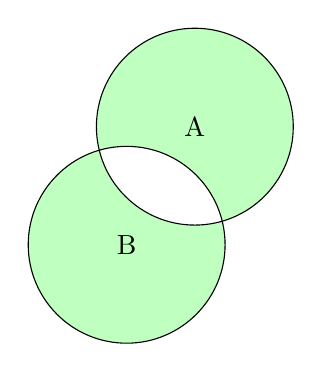
\begin{tikzpicture}
                {
    \def\firstcircle{(90:1cm) circle (1.25cm)}
    \def\secondcircle{(210:1cm) circle (1.25cm)}

    \fill[green!25] \firstcircle;
    \fill[green!25] \secondcircle;

    \begin{scope}
        \clip \firstcircle;
        \fill[white] \secondcircle;
    \end{scope}

    \draw \firstcircle node {A};
    \draw \secondcircle node {B};
}

                \end{tikzpicture}
            \end{multicols}
        \item Ausdruck für $A\Delta B\Delta C$:
            \begin{multicols}{2}
            \begin{align*}  &\mathbb{P}(A\Delta B\Delta C)=\\
                            &=\mathbb{P}(A)-\mathbb{P}(A\cap B)-\mathbb{P}(A\cap C)\\
                            &+\mathbb{P}(B)-\mathbb{P}(A\cap B)-\mathbb{P}(B\cap C)\\
                            &+\mathbb{P}(C)-\mathbb{P}(A\cap C)-\mathbb{P}(B\cap C)\\
                            &+4\mathbb{P}(A\cap B\cap C)\end{align*}
            \begin{align*}&\mathbb{P}(A\Delta B\Delta C)=\\&=\mathbb{P}(A)+\mathbb{P}(B)+\mathbb{P}(C)-2\mathbb{P}(A\cap B)-2\mathbb{P}(A\cap C)-2\mathbb{P}(B\cap C)+4\mathbb{P}(A\cap B\cap C)\end{align*}
                \columnbreak

                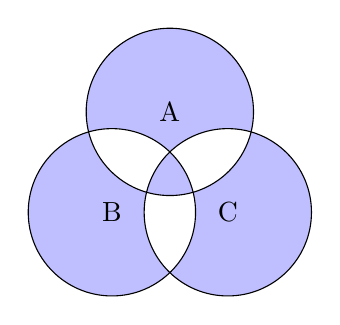
\begin{tikzpicture}[scale=0.85]
                    {
    \def\firstcircle{(90:1cm) circle (1.25cm)}
    \def\secondcircle{(210:1cm) circle (1.25cm)}
    \def\thirdcircle{(330:1cm) circle (1.25cm)}


    \fill[blue!25] \firstcircle;
    \fill[blue!25] \secondcircle;
    \fill[blue!25] \thirdcircle;

    \begin{scope}
        \clip \firstcircle;
        \fill[white] \secondcircle;
    \end{scope}
    \begin{scope}
        \clip \firstcircle;
        \fill[white] \thirdcircle;
    \end{scope}
    \begin{scope}
        \clip \secondcircle;
        \fill[white] \thirdcircle;
    \end{scope}

    \begin{scope}
        \clip \firstcircle;
        \clip \secondcircle;
        \fill[blue!25] \thirdcircle;
    \end{scope}

    \draw \firstcircle node {A};
    \draw \secondcircle node {B};
    \draw \thirdcircle node {C};
}

                \end{tikzpicture}
            \end{multicols}
            
            \textbf{Achtung:} da die Schnittmenge von $A\cap B\cap C$(also der Mittelpunkt) zur Symmetrischen Differenz dazugehört, folgt:
            $+4\mathbb{P}(A\cap B\cap C)$, da die Schnittmenge $3$-mal addiert wird, dann $6$-mal subtrahiert wird, muss sie folglich $4$-mal addiert werden. ($3x-6x+4x=1x$)
        \item Ausdruck für $n$-Mengen:
            \[\mathbb{P}(A_1\Delta A_2\Delta ...\Delta A_n)=\sum_{k=1}^n(-1)^{k-1}\cdot 2^{k-1}\cdot S_k\]
            \[\text{wobei } S_k=\sum_{1\leq i_1\leq i_2\leq ...\leq i_k \leq n}\mathbb{P}(A_{i_1}\cap A_{i_2}\cap ...\cap A_{i_k})\]
    \end{enumerate}
\end{Answer}
\end{uebsp}

\begin{uebsp}
\begin{Exercise}[label=ex:1.6]
In einer Urne sind 3 weiße und 2 schwarze Kugeln. Es wird eine Kugel gezogen und mit einer zusätzlichen Kugel der selben Farbe zurückgelegt (nach der ersten Ziehung sind also insgesamt 6 Kugeln in der Urne). Bestimmen Sie die Wahrscheinlichkeit, dass die zweite gezogene Kugel weiß ist.
\end{Exercise}
\begin{Answer}
    \begin{uebsp_theory}
        Mit der \reference{Bedingten Wahrscheinlichkeit}{Definition}{def:bedingte_wahrscheinlichkeit}\index{bedingte Wahrscheinlichkeit!Beispiel}
        \[\mathbb P(B|A)=\frac{\mathbb P(B)\mathbb P(A|B)}{\mathbb P(A)}\]
    \end{uebsp_theory}
    \begin{uebsp_theory}
        und dem \reference{Additionstheorem}{Satz}{satz:additionstheorem} \index{Additionstheorem!Beispiel}
        \[\mathbb P(\bigcup_{i=1}^n A_i)=\sum_{i=1}^n(-1)^{i-1}S_i\]
         folgt:
    \end{uebsp_theory}
\index{Additionstheorem!Beispiel}
\begin{enumerate}[1.]
    \item Schritt: die Wahrscheinlichkeit, dass bei 5 Kugeln beim 1. Schritt eine Weiße gezogen wird:
        \[\mathbb{P}(A)=\frac{3}{5}\;\Rightarrow\;\mathbb{P}(A^c)=\frac{2}{5}\;\leftarrow\fbox{\parbox[c][2em][c]{0.4\textwidth}{Wahrscheinlichkeit, dass eine schwarze Kugel gezogen wurde.}}\]
    \item Schritt: die Wahrscheinlichkeit, dass bei 6 Kugeln eine Weiße gezogen wird.
        \[\mathbb{P}(B|A)=\frac{4}{6}\cdot \frac{3}{5}\;\leftarrow\fbox{\parbox[c][2em][c]{0.4\textwidth}{Ereignisse paarweise unabhängig. \\$\Rightarrow$ Schnittmenge von beiden ist 0.}}\rightarrow\;\mathbb{P}(B|A^c)=\frac{3}{6}\cdot \frac{2}{5}\]
    \[\mathbb{P}(B)=\mathbb{P}(B|A)+\mathbb{P}(B|A^c)=\frac{2}{3}\cdot\frac{3}{5}+\frac{1}{2}\cdot \frac{2}{5}=\frac{3}{5}\]
        
\end{enumerate}
\end{Answer}
\end{uebsp}

\begin{uebsp}
\begin{Exercise}[label=ex:1.7]
Ein Würfel wird dreimal geworfen. Die Augenzahlen werden der Größe nach geordnet, die Zufallsvariable $X$ sei die mittlere (etwa $(2, 2, 5) \rightarrow 2$).\\
Bestimmen Sie die Verteilung von $X$.
\end{Exercise}
\begin{Answer}
    \begin{enumerate}[1.]
        \item Schritt: 4 Fälle betrachten:
                \begin{enumerate}[I)]
                    \item $y=X=z\;\Rightarrow\;$1 Permutation ($\dfrac{3!}{3!}$)
                    \item $y=X<z\;\Rightarrow\;$3 Permutationen ($\dfrac{3!}{2!}$)
                    \item $y<X=z\;\Rightarrow\;$3 Permutationen ($\dfrac{3!}{2!}$)
                    \item $y<X<z\;\Rightarrow\;$6 Permutationen ($\dfrac{3!}{1!}$)\\
                        z.B. kann $2<3<4$ durch folgende 6 Würfelkonstellationen/Permutationen entstehen:
                        $(2,3,4)$, $(2,4,3)$, $(3,2,4)$, $(3,4,2)$, $(4,2,3)$, $(4,3,2)$
                \end{enumerate}
        \item Schritt: Bestimmen der Wahrscheinlichkeit für X=k:
            \[X=1:\;1\cdot I+5\cdot II+0\cdot III+0\cdot IV=1\cdot1+5\cdot3+0\cdot3+0\cdot6=16\]
                \[\Rightarrow\mathbb{P}(X=1)=\frac{16}{216}\approx \;\;7.4\%\]
            \[X=2:\;1\cdot I+4\cdot II+1\cdot III+4\cdot IV=1\cdot1+4\cdot3+1\cdot3+4\cdot6=40\]
                \[\Rightarrow\mathbb{P}(X=2)=\frac{40}{216}\approx 18.5\%\]
            \[X=3:\;1\cdot I+3\cdot II+2\cdot III+6\cdot IV=1\cdot1+3\cdot3+2\cdot3+6\cdot6=52\]
                \[\Rightarrow\mathbb{P}(X=3)=\frac{52}{216}\approx 24.1\%\]
            \[X=4:\;1\cdot I+2\cdot II+3\cdot III+6\cdot IV=1\cdot1+2\cdot3+3\cdot3+6\cdot6=52\]
                \[\Rightarrow\mathbb{P}(X=4)=\frac{52}{216}\approx 24.1\%\]
            \[X=5:\;1\cdot I+1\cdot II+4\cdot III+4\cdot IV=1\cdot1+1\cdot3+4\cdot3+4\cdot6=40\]
                \[\Rightarrow\mathbb{P}(X=5)=\frac{40}{216}\approx 18.5\%\]
            \[X=6:\;1\cdot I+0\cdot II+5\cdot III+0\cdot IV=1\cdot1+0\cdot3+5\cdot3+0\cdot6=16\]
                \[\Rightarrow\mathbb{P}(X=6)=\frac{16}{216}\approx \;\;7.4\%\]
        \item Verteilungsfunktion $F_X(x)$:
            \begin{multicols}{2}

                \begin{tikzpicture}[scale=0.85]
                    {
    \begin{axis}[domain=0:8,
            axis x line=bottom, % no box around the plot, only x and y axis
            axis y line=left, % the * would suppress the arrow tips
            xlabel=Augenzahl,
            ylabel=Prozent,
            legend pos=north west,
            samples=50,
            height=6cm,
            width=10cm,
            clip=false]
            \addplot[blue] coordinates{(-1,0)(1,0)};
            \addlegendentry[align=left]{Vert.fkt. $f_X(x)$};%TODO: add a better label
            \addplot[blue,forget plot] coordinates{(1,7.4)(2,7.4)};
            \addplot[blue,forget plot] coordinates{(2,25.9)(3,25.9)};
            \addplot[blue,forget plot] coordinates{(3,50)(4,50)};
            \addplot[blue,forget plot] coordinates{(4,74.1)(5,74.1)};
            \addplot[blue,forget plot] coordinates{(5,92.6)(6,92.6)};
            \addplot[blue,forget plot] coordinates{(6,100)(8,100)};

            \draw[dotted] (axis cs:1,0) -- (axis cs:1,7.4);
            \draw[dotted] (axis cs:2,7.4) -- (axis cs:2,25.9);
            \draw[dotted] (axis cs:3,25.9) -- (axis cs:3,50);
            \draw[dotted] (axis cs:4,50) -- (axis cs:4,74.1);
            \draw[dotted] (axis cs:5,74.1) -- (axis cs:5,92.6);
            \draw[dotted] (axis cs:6,92.6) -- (axis cs:6,100);
            \addplot[discontinuityblue,forget plot] coordinates{(1,0)(2,7.4)(3,25.9)(4,50)(5,74.1)(6,92.6)};
            \addplot[continuityblue,forget plot] coordinates{(1,7.4)(2,25.9)(3,50)(4,74.1)(5,92.6)(6,100)};


            \addplot[red] coordinates{(-1,0)(1,0)};
            \addlegendentry[align=left]{Vert. diskret};%TODO: add better label
            \addplot[red,forget plot] coordinates{(1,7.4)(2,7.4)};
            \addplot[red,forget plot] coordinates{(2,18.5)(3,18.5)};
            \addplot[red,forget plot] coordinates{(3,24.1)(5,24.1)};
            \addplot[red,forget plot] coordinates{(5,18.5)(6,18.5)};
            \addplot[red,forget plot] coordinates{(6,7.4)(7,7.4)};
            \addplot[red,forget plot] coordinates{(7,0)(8,0)};

            \draw[dotted] (axis cs:1,0) -- (axis cs:1,7.4);
            \draw[dotted] (axis cs:2,7.4) -- (axis cs:2,18.5);
            \draw[dotted] (axis cs:3,18.5) -- (axis cs:3,24.1);
            \draw[dotted] (axis cs:5,24.1) -- (axis cs:5,18.5);
            \draw[dotted] (axis cs:6,18.5) -- (axis cs:6,7.4);
            \draw[dotted] (axis cs:7,7.4) -- (axis cs:7,0);

            \addplot[discontinuityred,forget plot] coordinates{(1,0)(2,7.4)(3,18.5)(5,24.1)(6,18.5)(7,7.4)};
            \addplot[continuityred,forget plot] coordinates{(1,7.4)(2,18.5)(3,24.1)(5,18.5)(6,7.4)(7,0)};
    \end{axis}
}

                \end{tikzpicture}

                Die rote Linie gibt die Verteilung diskret an, während die blaue Linie die Verteilungsfunktion $f_X(x)$ rechts darstellt.
            \columnbreak
            \[f_X(x) = \begin{cases} 
                        0 &\mbox{wenn } x < 1 \\
                        \frac{16}{216}\approx 7.4\% & \mbox{wenn } x < 2\\
                        \frac{56}{216}\approx 25.9\% & \mbox{wenn } x < 3\\
                        \frac{108}{216}\approx 50\% & \mbox{wenn } x < 4\\
                        \frac{160}{216}\approx 74.1\% & \mbox{wenn } x < 5\\
                        \frac{200}{216}\approx 92.6\% & \mbox{wenn } x < 6\\
                        \frac{216}{216}\approx 100\% & \mbox{wenn } x < 7 
                        \end{cases}\]
            \end{multicols}
    \end{enumerate}
\end{Answer}
\end{uebsp}



\newExercPage
\begin{uebsp}
\begin{Exercise}[label=ex:2.1]

    Die \reference{Poissonverteilung}{Kapitel}{sec:poissonverteilung} $\mathcal P(\lambda)$ hat die Wahrscheinlichkeitsfunktion \\

    \[p\left(x\right)=\frac{{\lambda }^{x}{e}^{-\lambda}}{x!}\left(x\geq 0\right)\]
 
Zeigen Sie, dass dies als Grenzwert der Wahrscheinlichkeitsfunktion der
\reference{Binomialverteilung}{Kapitel}{sec:binomialverteilung} mit $p = \frac{\lambda}{n}$, $ n \rightarrow \infty$ erhalten werden kann. \\



\end{Exercise}
\begin{Answer}
    \index{Binomialverteilung!Beispiel}
    \index{Poissonverteilung!Beispiel}
\begin{uebsp_theory} 
Die \reference{Binomialverteilung}{Kapitel}{sec:binomialverteilung} $\mathcal B(n,p)$:
\[p(x)={n\choose x}p^x(1-p)^{n-x}.\]
und der \reference{Binomialkoeffizient}{Anhang}{sec:binomialkoeffizient}
\[{n\choose k} = \frac{n!}{k!(n-k)!}\]
\end{uebsp_theory}

Demnach: \\

\[\mathcal B(k | n,p) = {n\choose k}p^k(1-p)^{n-k} = \textbf{wir ersetzen $p$ durch $\frac{\lambda}{n}$ } = {n\choose k}(\frac{\lambda}{n})^k(1-\frac{\lambda}{n})^{n-k}\]
\[=\frac{n!}{k!(n-k)!} (\frac{\lambda}{n})^k(1-\frac{\lambda}{n})^{n-k} = \frac{n(n-1)(n-2)...(n-k+1)((n-k)!)}{k!(n-k)!}\frac{\lambda{^k}}{n^{k}}(1-\frac{\lambda}{n})^{n-k} =\]
\[\frac{n(n-1)(n-2)...(n-k+1)}{n^{k}}\frac{\lambda{^k}}{k!}(1-\frac{\lambda}{n})^{n-k}\]
Betrachten wir nun zuerst den linken Teil des Ausdrucks: 
\[\frac{n}{n}\frac{n-1}{n}\frac{n-2}{n}\dots \frac{n-k+1}{n} = 1*(1-\frac{1}{n})(1-\frac{2}{n}) * \dots * (1-\frac{k+1}{n})\]
Bilden wir nun davon den $\lim_{n \to \infty}$ vereinfacht sich der linke Teilausdruck zu $1$.

Nun betrachten wir den verbleibenden rechten Teilausdruck
\[\frac{\lambda^{k}}{k!}(1-\frac{\lambda}{n})^{n-k} = \frac{\lambda^{k}}{k!}(1-\frac{\lambda}{n})^{n} (1-\frac{\lambda}{n})^{-k}\]
Bilden wir nun auch hier den $\lim_{n \to \infty}$ wird $(1-\frac{\lambda}{n})^{-k}$ zu 1. Mit dem Wissen, dass:
\begin{uebsp_theory} 
$e^{x} = \lim_{n \to \infty}(1+\frac{x}{n})^{n}$
\end{uebsp_theory}

Erhalten wir, wie erhofft:
\[\lim_{n \to \infty} B(k | n,\frac{\lambda}{n}) = p\left(k\right)=\frac{{\lambda }^{k}{e}^{-\lambda}}{k!}\]
\end{Answer}
\end{uebsp}

\begin{uebsp}
\begin{Exercise}[label=ex:2.2]
Es sei \\ 
\[ F(x) = \left\{
  \begin{array}{l l}
    0 & \quad \text{für $x < 0$}\\
    \frac{{x}^{2}}{4}  & \quad \text{für $0 \le x < 1$} \\
    \frac{x}{2} & \quad \text{für $1 \le x < 2$} \\
    1 & \quad \text{für $x \ge 2$}
  \end{array} \right.\]
\Question
Zeigen Sie, dass $F$ eine Verteilungsfunktion ist.
\Question
$X$ sei nach $F$ verteilt. Bestimmen Sie $\mathbb{P}(X < 1)$, $\mathbb{P}(X \le 1)$, $\mathbb{P}(X = 0$),$\mathbb{P}(X = 1)$, $\mathbb{P}(X = 2)$.
\end{Exercise}
\begin{Answer}
    \index{Verteilungsfunktion!Eigenschaften!Beispiel}
\begin{enumerate}[(a)]
    \item{
        Die Kriterien für eine \reference{Verteilungsfunktion}{Definition}{def:verteilungsfunktion_eigenschaften} lauten:
    	\begin{uebsp_theory}
    	$F:\mathbb R\to\mathbb R$ ist genau dann eine Verteilungsfunktion, wenn
    	\begin{enumerate}
    	\item $0\le F(x)\le 1$ für alle $x$,
    	\item $F$ ist monoton nichtfallend,
    	\item $F$ ist rechtsstetig,
    	\item $\lim_{x\to-\infty}F(x)=0$,
    	\item $\lim_{x\to\infty}F(x)=1$.
    	\end{enumerate}
    	\end{uebsp_theory}
    	
    	Wie wir sehen sind die Punkte alle erfüllgt:
    	
    	\begin{enumerate}
    	\item  \checkmark : Die Werte die $x^{2}$ (bei $0 \le x < 1$) annehmen kann liegen im Bereich [0;1[ selbes gilt für $\frac{x^{2}}{4}$. Auch die Werte für $\frac{x}{2}$ (bei $1 \le x < 2$ ) liegen im Bereich [0,5;1[.
    	\item  \checkmark : Sowohl  $\frac{x^{2}}{4}$ als auch $\frac{x}{2}$ sind monoton steigend.
    	\item \checkmark : erfüllt
    	\item \checkmark : erfüllt
    	\item \checkmark : erfüllt
    	\end{enumerate}
    	
    	
    }
  
\item Diese Wahrscheinlichkeiten lassen sich am besten aus der Verteilungsfunktion berechnen:
    \index{Wahrscheinlichkeiten mit Verteilungsfunktion!Beispiel}
    \begin{uebsp_theory}
        Mit den \reference{Wahrscheinlichkeiten mithilfe der Verteilungsfunktion}{Kapitel}{sec:wahrscheinlichkeiten_verteilungsfunktionen} folgt:
        \[\mathbb P(X\le a)=F_X(a),\]
        \[\mathbb P(X<a)=F_X(a-0),\]
        \[\mathbb P(a< X\le b)=F_X(b)-F_X(a),\]
        \[\mathbb P(a< X< b)=F_X(b-0)-F_X(a),\]
        \[\mathbb P(a\le X\le b)=F_X(b)-F_X(a-0),\]
        \[\mathbb P(a\le X< b)=F_X(b-0)-F_X(a-0).\]
        \[\mathbb P( X= a)=F_X(a)-F_X(a-0).\]
    Dabei ist $F(x-0)=\lim_{h\downarrow 0}F(x-h)$ der linksseitige Grenzwert
    von $F$ in $x$. \\
    \end{uebsp_theory}
    
    Daraus ergibt sich für unser Beispiel: \\
   	\begin{itemize}
   	\item $\mathbb{P}(X < 1)=F_X(1-0)=\frac{1}{4}$
   	\item $\mathbb{P}(X \le 1)=F_X(1)=\frac{1}{2}$
   	\item $\mathbb{P}(X = 0)=F_X(0)-F_X(0-0)=\frac{0^{2}}{4}-0=0$
   	\item $\mathbb{P}(X = 1)=F_X(1)-F_X(1-0)=\frac{1}{2}-\frac{1^{2}}{4}=\frac{1}{4}$
   	\item $\mathbb{P}(X = 2)=F_X(2)-F_X(2-0)=1-\frac{2}{2}=0$
   	\end{itemize}
    
\end{enumerate}
\end{Answer}
\end{uebsp}

\begin{uebsp}
\begin{Exercise}[label=ex:2.3]
$X$ und $Y$ seien unabhängig poissonverteilt mit Parameter $\lambda$ und $\mu$. Bestimmen Sie die Verteilung von $X + Y$.
\end{Exercise}
\begin{Answer}
    \index{Poissonverteilung!Beispiel}
    \index{Unabhängigkeit!Verteilung!Beispiel}
    \index{Faltung von Dichten!Beispiel}
\begin{uebsp_theory}
    Die Wahrscheinlichkeitsfunktion der \reference{Poissonverteilung}{Kapitel}{sec:poissonverteilung} ist wie folgt definiert:
    \[{\lambda^xe^{-\lambda}\over x!}\]
    Für zwei \reference{unabhängigie Zufallsvariablen $(X,Y)$}{Definition}{def:unabhaengigkeit_verteilung} gilt: 
    \[p(x)=F_{X,Y}(x,y)=F_{X}(x)\cdot F_Y(y).\]

    Außerdem gilt, für \reference{die gemeinsame Dichte}{Satz}{satz:faltung_dichten}: 
    \[f_{x+y}=\underbrace{f_X*f_Y(z)}_{\text{Faltung}}=\int_{-\infty}^{\infty}f_X(x)\cdot f_Y(z-x)dx\]
\end{uebsp_theory}

Aus der Angabe wissen wir also:
\[p(x) = {\lambda^xe^{-\lambda}\over x!}\text{ und }p(y) = {\mu^ye^{-\mu}\over y!}\]
Wir führen eine neue Variable ein: $Z=X+Y \Rightarrow Y=Z-X$ \\

$\mathbb{P}(Z=z)=\mathbb{P}(X+Y=z)=\sum_x\mathbb{P}(X=x,Y=z-x)$\\ \\
Da die Varaiblen unabhängig sind ergibt das: \\ $\sum_{x}\mathbb{P}(X=x,Y=z-x)=\sum_{x}[p(x)p(z-x)] \text{ was der Faltung entspricht.}$\\ 

$=\sum_{x=0}^{z}{\lambda^xe^{-\lambda}\over x!}\cdot{\mu^{(z-x)}e^{-\mu}\over (z-x)!}=e^{-\lambda-\mu} \cdot  \sum_{x=0}^{z} \frac{1}{x! \cdot (z-x)!} \cdot \lambda^{z} \cdot  \mu^{z-x} = e^{-\lambda-\mu} \cdot \sum_{x=0}^{z}  \cdot {z \choose x} \cdot \frac{1}{z!} \cdot \lambda^{z} \cdot  \mu^{z-x} = \frac{e^{-\lambda-\mu}}{z!}\sum_{x=0}^{z} {z \choose x} \cdot  \lambda^{z} \cdot  \mu^{z-x} = \frac{e^{-\lambda-\mu}}{z!}\sum_{x=0}^{z}  {z \choose x} \cdot \lambda^{z} \cdot  \mu^{z-x}$ 
\\ \\
Mit Hilfe des \reference{Binomischen Lehrsatzes}{Anhang}{sec:binom_lehrsatz} $(a+b)^n=\sum_{k=0}^n~{n\choose k} \cdot a^{n-k} \cdot b^k$ lässt sich dies weiter vereinfachen zu: \\ \\
$p(z) = \frac{(\lambda +\mu)^{z} \cdot e^{-(\lambda+\mu)}}{z!}$\\

Dies entspricht wiederum einer Poisson-Verteilung von Z.

\end{Answer}
\end{uebsp}

\begin{uebsp}
\begin{Exercise}[label=ex:2.4]
$X$ und $Y$ seien unabhängig gleichverteilt auf $[0, 1]$. Bestimmen Sie die Verteilung von $X + Y$ .
\end{Exercise}
\begin{Answer}
    \index{Gleichverteilung!Beispiel}
    \index{Unabhängigkeit!Verteilung!Beispiel}
    \index{Faltung von Dichten!Beispiel}

\begin{uebsp_theory}
    Die Wahrscheinlichkeitsfunktion der \reference{diskreten Gleichverteilung}{Kapitel}{sec:gleichverteilung_diskret} ist wie folgt definiert:
    \[\frac{1}{b-a}\;\;\forall a\leq x\leq b\]
    Für zwei \reference{unabhängigie Zufallsvariablen $(X,Y)$}{Definition}{def:unabhaengigkeit_verteilung} gilt: 
    \[p(x)=F_{X,Y}(x,y)=F_{X}(x)\cdot F_Y(y).\]

    Außerdem gilt, für \reference{die gemeinsame Dichte}{Satz}{satz:faltung_dichten}: 
    \[f_{x+y}=\underbrace{f_X*f_Y(z)}_{\text{Faltung}}=\int_{-\infty}^{\infty}f_X(x)\cdot f_Y(z-x)dx\]
\end{uebsp_theory}

D.h.: als Ausgangssituation haben wir:
\[ f_X(x) = \left\{
  \begin{array}{l l}
    1 & \quad \text{für $x \in [0,1]$}\\
    0 & \quad \text{sonst}
  \end{array} \right.\]
  
\[ f_Y(y) = \left\{
    \begin{array}{l l}
      1 & \quad \text{für $y \in [0,1]$}\\
      0 & \quad \text{sonst}
    \end{array} \right.\]

Wir führen eine neue Variable ein: $Z=X+Y \Rightarrow Y=Z-X \Rightarrow z \in [0,2]$

\begin{uebsp_theory}
    Wenn die gemeinsame Verteilung diskret bzw. stetig ist, kann man in dieser
    Definition von den zwei Zufallsvariablen(vorher) die Verteilungsfunktion durch die Wahrscheinlichkeits- bzw. Dichte-
    funktion ersetzen:
    \[f_{X,Y}(x,y)=f_{X}(x)\cdot f_Y(y).\]
    \reference{}{Definition}{def:unabhaengigkeit_verteilung}
\end{uebsp_theory}

$f_{X,Y}=\int_{-\infty}^{\infty}f_X(x)f_Y(z-x)dx = f_Z(z)$ \\
Wir betrachten nur das Integral von $0$ bis $1$ da außerhalb $f_X(x)=0$ für alle gilt:\\
$f_Z(z) = \int_{0}^{1} \underbrace{f_X(x)}_{=1}f_Y(z-x)dx  $\\ \\
Innerhalb des Intervalls [0,1] ist $f_X(x)=1$ für alle x. \\
$f_Z(z)=\int_{0}^{1}f_Y(z-x)dx$ \\
Da $y \in [0,1] \Rightarrow (z-x) \in [0,1] $ dies führt auf 2 Fälle:

\begin{enumerate}
\item{$z \in [0,1[:  z-x \ge 0\Rightarrow z \ge x $ \\ \\ $f_{(X+Y)_1}(z)=\int_{0}^{z}1dx=z$ } 
        \item{$z \in [1,2[: z-x  \le 1 \text{ damit } f_Y = 1\\ z-1\le x$\\
$f_{(X+Y)_2}(z)=\int_{z-1}^{1}1dx=1-(z-1)=2-z$} 
\end{enumerate}

Insgesamt ergibt sich also:\\ \\


\[ f_{X+Y}(z) = \left\{
    \begin{array}{l l}
      z & \quad \text{für $0 \le z < 1$}\\
      2-z & \quad \text{für $1 \le z <2$}\\
      0 & \quad \text{sonst}
    \end{array} \right.\]

\end{Answer}
\end{uebsp}

\begin{uebsp}
\begin{Exercise}[label=ex:2.5]
$X$ sei gleichverteilt auf $[0, 1]$. Bestimmen Sie die Verteilung von $-\log X$.
\end{Exercise}
\begin{Answer}
    \index{Gleichverteilung!Beispiel}

Laut Skriptum:\\
Wenn die gemeinsame Verteilung diskret bzw.\ stetig ist, kann man
in dieser Definition die Verteilungsfunktion durch die Wahrscheinlichkeits-
bzw.\ Dichtefunktion ersetzen. 

\begin{uebsp_theory}
    \textbf{Transformationssatz für Dichten}\index{Transformationssatz für Dichten!Beispiel}\\
$X=(X_1,\dots,X_n)$ sei stetig verteilt mit der Dichte $f_X$.
$g:\mathbb R^n\to\mathbb R^n$ sei stetig differenzierbar und 
eindeutig umkehrbar. $Y=g(X)$ (d.h.\ $Y_i=g_i(X_1,\dots, X_n)$)
ist dann ebenfalls stetig verteilt mit der Dichte
\[f_Y(y)=\begin{cases}f_X(g^{-1}(y))|{\partial g^{-1}\over\partial y}(y)|=f_X(g^{-1}(y)){1\over |{\partial g\over\partial x}(g^{-1}(y))|} &\mbox{wenn } y \in g(\mathbb{R}^n), \\
0 & \mbox{sonst.}\end{cases}\]
Dabei ist
\[{\partial g\over\partial x}=\det( ({\partial g_i\over\partial x_j})_{n\times
n})\]
die Funktionaldeterminate.
\end{uebsp_theory}

$Y = g(x) = -log(x)  = -ln(x)\\$
$-Y = ln(x)\\$
$x=e^{-y}=g^{-1}(y)\\$

$F_{Y}(y)=\mathbb{P}(Y \le y)=\mathbb{P}(-ln(x) \le y)=\mathbb{P}(x \ge e^{-y})=e^{-y} \textbf{???}\\\\$

$f_Y(y)=f_X(g^{-1}(y)) \cdot \vert((g^{-1})')\vert=f_X(g^{-1}(y)) \cdot \vert((e^{-y})')\vert=f_X(g^{-1}(y)) \cdot \vert-e^{-y}\vert=\\$
$f_Y(y)=f_X(g^{-1}(y)) \cdot e^{-y}$


\[ f_X(x) = \left\{
  \begin{array}{l l}
    1 & \quad \text{$x \in [0,1]$}\\
    0 & \quad \text{sonst} \\
\end{array} \right.\]

Mit $f_X(x)$ eingesetzt in $f_Y(y)$ folgt: \\

\[ f_Y(y) = \left\{
  \begin{array}{l l}
    e^{-y} & \quad \text{$0 \le g^{-1}(y) \le 1$}\\
    0 & \quad \text{sonst} \\
\end{array} \right.\]

Wobei das aber keine richtige Einschränkung ist, denn $g^{-1}(y)=e^{-y}$ ist sowieso immer kleiner als 1 für $x \in [0,1]$

\end{Answer}
\end{uebsp}

\begin{uebsp}
\begin{Exercise}[label=ex:2.6]
$X$ und $Y$ haben eine gemeinsame Verteilung mit der Dichte \\
\[ f(x,y) = \left\{
  \begin{array}{l l}
    $c(x+y)$ & \quad \text{für $0 \le x$, $y \le 1$}\\
    0  & \quad \text{sonst} \\
  \end{array} \right.\]
Bestimmen $c$ und die Randdichten von $X$ und $Y$.
\end{Exercise}
\begin{Answer}
Eigenschaften der gemeinsamen Dichtefunktion: \\

...\\

Mit dem 2. Punkt folgt: \\
$\int\limits_{-\infty}^\infty \int\limits_{-\infty}^\infty f_{XY}(x,y)dxdy=1$ \\
Da sowohl x als auch y nur im Intervall [0,1] interessant sind, kann man die Integralgrenzen einschränken:\\

$\int\limits_{0}^{1} \int\limits_{0}^{1} f_{XY}(x,y)dxdy=\int\limits_{0}^{1} \int\limits_{0}^{1} c \cdot (x+y)dxdy = 1$\\
$c \cdot \int\limits_{0}^{1} \int\limits_{0}^{1} (x+y)dxdy$\\
$c \cdot \int\limits_{0}^{1}( \frac{x^2}{2}+xy )|_{x=0}^{1} dy$\\
$c \cdot \int\limits_{0}^{1} (\frac{1}{2}+y )dy = c \cdot (\frac{y}{2}+\frac{y^2}{2})|_{y=0}^{1} = c \cdot (\frac{1}{2}+\frac{1}{2})=c \Rightarrow c=1$\\ \\

Die Randdichten von X und Y sind definiert durch:

\begin{itemize}
\item $f_X(x)=\int\limits_{-\infty}^\infty f_{XY}(x,y)dy$
\item $f_Y(y)=\int\limits_{-\infty}^\infty f_{XY}(x,y)dx$
\end{itemize} 

Randdichte von X:\\
$f_X(x)=\int\limits_{-\infty}^\infty f_{XY}(x,y)dy = c \cdot \int\limits_{0}^1 (x+y) dy = c \cdot (xy + \frac{y^2}{2})|_{0}^1 = c \cdot (x+\frac{1}{2}) \textbf{ und mit c=1 folgt:}\\ f_X(x)= (x+\frac{1}{2})$ \\

Randdichte von Y:\\
$f_Y(y)=\int\limits_{-\infty}^\infty f_{XY}(x,y)dx =c \cdot \int\limits_{0}^1 (x+y) dx = c \cdot (\frac{x^2}{2} + xy )|_{0}^1 = c \cdot (y+\frac{1}{2})= (y+\frac{1}{2}) $\\



\end{Answer}
\end{uebsp}

\begin{Exercise}[label=ex:2.7]
Ein Würfel wird dreimal geworfen. X sei die größte der drei Augenzahlen, Y die kleinste. Bestimmen Sie die gemeinsame Verteilung von X und Y und die beiden Randverteilungen. \\
\end{Exercise}
\begin{Answer}
\end{Answer}


\newExercPage
\begin{uebsp}
\begin{Exercise}[label=ex:3.1]
$X$ und $Y$ seien unabhängig gammaverteilt mit Parametern $(\alpha, \lambda)$ und
$(\beta, \lambda)$. Zeigen Sie, dass $S = X + Y$ ebenfalls gammaverteilt ist.
\end{Exercise}
\begin{Answer}
z.z. die Reproduktivität von $X$ und $Y$ mit $(\alpha, \lambda)$ und $(\beta, \lambda)\Rightarrow \Gamma_{\alpha,\lambda}*\Gamma_{\beta,\lambda}=\Gamma_{\alpha+\beta,\lambda}$.
\begin{uebsp_theory}
    Mit dem \reference{Satz}{Satz}{satz:verteilung_x_y} gilt: (kommt aus \reference{Transformationssatz für Dichten}{Kapitel}{sec:transformationssatz_dichten}\index{Transformationssatz für Dichten!Beispiel}):
    \[f_{X+Y}(z)=f_X*f_Y(z)=\int_{-\infty}^{\infty} f_X(x)f_Y(z-x)dx.\]
\end{uebsp_theory}

\begin{uebsp_theory}
    und der \reference{Gammaverteilung}{Kapitel}{sec:gammaverteilung} $\Gamma(\alpha, \lambda)$:\index{Gammaverteilung!Beispiel}
        \[f(x) = \begin{cases} 
                    \frac{\lambda^\alpha x^{\alpha-1}}{\Gamma(\alpha)}e^{-\lambda\; x} &\mbox{wenn } x \geq 1 \\
                    0 & \mbox{sonst}
            \end{cases}\]
    folgt:
\end{uebsp_theory}

Einführen der Variable $S=x+y\Rightarrow y=S-x$

\begin{eqnarray*}
f_{\Gamma_{\alpha,\lambda}*\Gamma_{\beta,\lambda}} &=& \int_0^S f_{\Gamma_{\alpha, \lambda}}(x) \cdot f_{\Gamma_{\beta, \lambda}}(x)dx \\
 &=& \int_0^S\frac{\lambda^\alpha x^{\alpha-1}}{\Gamma(\alpha)}\cdot e^{-\lambda x}\cdot \frac{\lambda^{\beta}(S-x)^{\beta-1}}{\Gamma(\beta)}e^{-\lambda(S-x)}dx \\
 &=& \frac{\lambda^{\beta+\alpha}}{\Gamma(\alpha)\Gamma(\beta)} \int_0^S x^{\alpha-1}\cdot \cancel{e^{-\lambda x}}\cdot (S-x)^{\beta-1} e^{-\lambda S} \cancel{e^{\lambda x}}dx\\
 &=& \frac{\lambda^{\beta+\alpha}}{\Gamma(\alpha)\Gamma(\beta)}\cdot e^{-\lambda S} \int_0^S x^{\alpha-1}\cdot (S-x)^{\beta-1} dx\\
 &=& \frac{\lambda^{\beta+\alpha}}{\Gamma(\alpha)\Gamma(\beta)}\cdot e^{-\lambda S} \int_0^S \left(\frac{S\cdot x}{S}\right)^{\alpha-1}\cdot \left(S\left(1-\frac{x}{S}\right)\right)^{\beta-1} dx\\
 &=& \frac{\lambda^{\beta+\alpha}S^{\alpha-1}S^{\beta-1}}{\Gamma(\alpha)\Gamma(\beta)}\cdot e^{-\lambda S} \int_0^S \left(\frac{x}{S}\right)^{\alpha-1}\cdot \left(1-\frac{x}{S}\right)^{\beta-1} dx\\
\end{eqnarray*}
Anschließend wird $u=\dfrac{x}{S}$ substituiert: $\Rightarrow\dfrac{du}{dx}=\dfrac{1}{S}$\\\\
Für die Grenze $S$ gilt: $\dfrac{S}{S}=1$, da wir statt $x$ das $S$ einsetzen.

\begin{uebsp_theory}
Die Betafunktion ist definiert als:
%TODO: copy this definition to scriptum
%TODO: don't forget to index as example
\[\beta(x,y)=\int_0^1t^{x-1}(1-t)^{y-1}dt=\frac{\Gamma(x)\cdot\Gamma(y)}{\Gamma(x+y)}\]
\end{uebsp_theory}

\begin{eqnarray*}
f_{\Gamma_{\alpha,\lambda}*\Gamma_{\beta,\lambda}} &=& \frac{\lambda^{\beta+\alpha}S^{\alpha-1}S^{\beta-1}}{\Gamma(\alpha)\Gamma(\beta)}\cdot e^{-\lambda S} \int_0^1 u^{\alpha-1}\cdot (1-u)^{\beta-1} du\cdot \frac{1}{S^{-1}}\\
 &=& \frac{\lambda^{\beta+\alpha}S^{\alpha-1}S^{\beta-1}}{\Gamma(\alpha)\Gamma(\beta)}\cdot e^{-\lambda S} \beta(\alpha, \beta)\cdot \frac{1}{S^{-1}}\\
 &=& \frac{\lambda^{\beta+\alpha}S^{\alpha-1}S^{\beta\cancel{-1}}}{\Gamma(\alpha)\Gamma(\beta)\cancel{S^{-1}}}\cdot e^{-\lambda S} \frac{\Gamma(\alpha)\cdot\Gamma(\beta)}{\Gamma(\alpha+\beta)}\\
 &=& \frac{\lambda^{\beta+\alpha}S^{\alpha+\beta-1}}{\cancel{\Gamma(\alpha)}\cdot\cancel{\Gamma(\beta)}}\cdot e^{-\lambda S} \frac{\cancel{\Gamma(\alpha)}\cdot\cancel{\Gamma(\beta)}}{\Gamma(\alpha+\beta)}\\
 &=& \frac{\lambda^{\beta+\alpha}S^{\alpha+\beta-1}}{\Gamma(\alpha+\beta)}\cdot e^{-\lambda S} = f_{\Gamma_{(\alpha+\beta),\lambda}}\\
f_{\Gamma_{\alpha,\lambda}*\Gamma_{\beta,\lambda}} &=& f_{\Gamma_{(\alpha+\beta),\lambda}}\;\;\fbox{ q.e.d.}\\
\end{eqnarray*}

\end{Answer}
\end{uebsp}

\begin{uebsp}
\begin{Exercise}[label=ex:3.2]
$X$ und $Y$ seien unabhängig gammaverteilt mit Parametern $(\alpha, \lambda)$ und
$(\beta, \lambda)$. Zeigen Sie, dass $Q = X/(X + Y)$ betaverteilt ist (für Wagemutige:
bestimmen Sie die gemeinsame Dichte von $S$ und $Q$ und zeigen Sie, dass sie unabhängig sind).
\end{Exercise}
\begin{Answer}
\begin{uebsp_theory}
Mit der \reference{Gammaverteilung}{Kapitel}{sec:gammaverteilung} $\Gamma(\alpha, \lambda)$:\index{Gammaverteilung!Beispiel}
    \[f(x) = \begin{cases} 
                \frac{\lambda^\alpha x^{\alpha-1}}{\Gamma(\alpha)}e^{-\lambda\; x} &\mbox{wenn } x \geq 1 \\
                0 & \mbox{sonst}
                \end{cases}\]
\end{uebsp_theory}

\begin{uebsp_theory}
    und dem \reference{Transformationssatz für Dichten}{Kapitel}{sec:transformationssatz_dichten}\index{Transformationssatz für Dichten!Beispiel}
    \[f_Y(y)=\begin{cases}f_X(g^{-1}(y))|{\partial g^{-1}\over\partial y}(y)| &\mbox{wenn } y \in g(\mathbb{R}^n), \\
    0 & \mbox{sonst.}\end{cases}\]
    folgt:
\end{uebsp_theory}

Mit $g(x,y)=\left( \begin{array}{c} \frac{x}{x+y} \\ x \end{array} \right)$ (wobei hier $oben=Q$ und $unten=x$ gilt), der Umkehrfunktion $g^{-1}(Q,x)=\left( \begin{array}{c} x \\ \frac{x}{Q}-x \end{array} \right)$ ($oben=x$, $unten=y$) und den \reference{Determinantenrechenregeln}{Anhang}{sec:determinante_2_2} folgt:

%TODO: eventuell stimmt hier im ganzen beispiel x und y nicht ganz .....
\begin{align*}\left|\frac{\partial g^{-1}}{\partial y}(y)\right|&=\left|det\left|\begin{array}{cc}\frac{\partial g_1^{-1}}{\partial x} & \frac{\partial g_1^{-1}}{\partial Q} \\ \frac{\partial g_2^{-1}}{\partial x} & \frac{\partial g_2^{-1}}{\partial Q} \end{array}\right|\right| = \left|det\left|\begin{array}{cc}\frac{\partial x}{\partial x} & \frac{\partial x}{\partial Q} \\ \frac{\partial \frac{x}{Q}-x}{\partial x} & \frac{\partial \frac{x}{Q}-x}{\partial Q} \end{array}\right|\right| = \left|det\left|\begin{array}{cc}1 & 0 \\ \frac{1}{Q}-1 & -\frac{x}{Q^2} \end{array}\right|\right|=\\
&=\left|-\frac{x}{Q^2}\right|=\frac{x}{Q^2}
\end{align*}

\begin{eqnarray*}
f_a &=& \int_{-\infty}^\infty f_{\Gamma_{\alpha, \lambda}}\cdot f_{\Gamma_{\beta, \lambda}}\cdot \left|\frac{\partial g^{-1}}{\partial y}(y)\right| dx\\
 &=& \int_{-\infty}^\infty \frac{\lambda^\alpha x^{\alpha-1}}{\Gamma(\alpha)}e^{-\lambda\; x} \cdot \frac{\lambda^\beta y^{\beta-1}}{\Gamma(\beta)}e^{-\lambda\; y}\cdot \frac{x}{Q^2} dx \;\;\fbox{wobei hier gilt: $y\;=\;y(x)$}\\
 &=& \int_{-\infty}^\infty \frac{\lambda^\alpha x^{\alpha-1}}{\Gamma(\alpha)}e^{-\lambda\; x} \cdot \frac{\lambda^\beta \left(\frac{x}{Q}-x\right)^{\beta-1}}{\Gamma(\beta)}e^{-\lambda(\; \frac{x}{Q}-x)}\cdot \frac{x}{Q^2} dx \;\;\fbox{ mit $y=\dfrac{x}{Q}-x$.}\\
 &=& \frac{\lambda^\alpha\cdot \lambda^\beta}{\Gamma(\alpha)\cdot \Gamma(\beta)}\int_{-\infty}^\infty x^{\alpha-1}\cancel{e^{-\lambda\; x}} \cdot \left(\frac{x}{Q}-x\right)^{\beta-1}e^{-\frac{\lambda\;x}{Q}}\cancel{e^{\lambda\;x}}\cdot \frac{x}{Q^2} dx\\
 &=& \frac{\lambda^\alpha\cdot \lambda^\beta}{\Gamma(\alpha)\cdot \Gamma(\beta)}\int_{-\infty}^\infty x^{\alpha-1} \cdot \left(x\left(\frac{1}{Q}-1\right)\right)^{\beta-1}e^{-\frac{\lambda\;x}{Q}}\cdot \frac{x}{Q^2} dx\\
 &=& \frac{\lambda^\alpha\cdot \lambda^\beta}{\Gamma(\alpha)\cdot \Gamma(\beta)}\int_{-\infty}^\infty x^{\alpha-1} \cdot x^{\beta-1}\cdot \left(\frac{1}{Q}-1\right)^{\beta-1}e^{-\frac{\lambda\;x}{Q}}\cdot \frac{x}{Q^2} dx\\
\end{eqnarray*}
Anschließend wird $u=\dfrac{x}{Q}\cdot \lambda\Rightarrow x=\dfrac{Q}{\lambda}\cdot u$ Substituiert. (Außerdem: $\dfrac{du}{dx}=\dfrac{\lambda}{Q}\Rightarrow dx=\dfrac{Q}{\lambda}\cdot du$)

\begin{uebsp_theory}
Die Gammafunktion ist definiert als:
%TODO: copy this definition to scriptum
%TODO: don't forget to index as example
\[\Gamma(x)=\int_0^\infty x^{t-1}e^{-x}dx=(z-1)\Gamma(z-1)\]
\end{uebsp_theory}

\begin{eqnarray*}
f_a &=& \frac{\lambda^\alpha\cdot \lambda^\beta}{\Gamma(\alpha)\cdot \Gamma(\beta)}\int_{-\infty}^\infty \left(\frac{Q}{\lambda}\right)^{\alpha-1}u^{\alpha-1} \cdot \left(\frac{Q}{\lambda}\right)^{\beta-1}u^{\beta-1}\cdot \left(\frac{1}{Q}-1\right)^{\beta-1}e^{-u}\cdot \frac{\cancel{Q}\;u}{\lambda\;\cancel{Q}^{\cancel{2}}} \dfrac{\cancel{Q}}{\lambda} \cdot du\\
 &=& \frac{\lambda^{\alpha+\beta}}{\Gamma(\alpha)\cdot \Gamma(\beta)}\int_{-\infty}^\infty Q^{\alpha-1}\cdot u^{\alpha-1} \cdot Q^{\beta-1}\cdot u^{\beta-1}\cdot \left(\frac{1}{Q}-1\right)^{\beta-1}e^{-u}\cdot u\cdot \lambda^{-2}\cdot \lambda^{-\beta+1}\cdot \lambda^{-\alpha+1} \cdot du\\
 &=& \frac{\lambda^{\cancel{\alpha}+\cancel{\beta}-\cancel{\alpha}+1-\cancel{\beta}+1-2}}{\Gamma(\alpha)\cdot \Gamma(\beta)}\int_{-\infty}^\infty Q^{\alpha-1}\cdot u^{\alpha-1} \cdot u^{\beta-1}\cdot  Q^{\beta-1}\cdot \left(\frac{1}{Q}-1\right)^{\beta-1}e^{-u}\cdot u \cdot du\\
 &=& \frac{\lambda^{1+1-2}}{\Gamma(\alpha)\cdot \Gamma(\beta)}\int_{-\infty}^\infty Q^{\alpha-1}\cdot u^{\alpha+\beta-2}\cdot u\cdot \left(\frac{Q}{Q}-Q\right)^{\beta-1}e^{-u}\cdot du\\
 &=& \frac{1}{\Gamma(\alpha)\cdot \Gamma(\beta)}\int_{-\infty}^\infty Q^{\alpha-1}\cdot u^{\alpha+\beta-1}\cdot \left(1-Q\right)^{\beta-1}e^{-u} \cdot du\\
 &=& \frac{Q^{\alpha-1}\cdot \left(1-Q\right)^{\beta-1}}{\Gamma(\alpha)\cdot \Gamma(\beta)}\int_{-\infty}^\infty u^{\alpha+\beta-1}\cdot e^{-u} \cdot du\;\;\fbox{ einsetzen der Gammafunktion}\\
f_a &=& \frac{Q^{\alpha-1}\cdot \left(1-Q\right)^{\beta-1}}{\Gamma(\alpha)\cdot \Gamma(\beta)}\cdot \Gamma(\alpha+\beta)
\end{eqnarray*}

\begin{uebsp_theory}
Die Betafunktion ist definiert als:
%TODO: copy this definition to scriptum
%TODO: don't forget to index as example
\[\beta(x,y)=\int_0^1t^{x-1}(1-t)^{y-1}dt=\frac{\Gamma(x)\cdot\Gamma(y)}{\Gamma(x+y)}\]
\end{uebsp_theory}

\begin{uebsp_theory}
Die \reference{Betaverteilung 1. Art}{Kapitel}{sec:betaverteilung_first} $\beta(\alpha, \lambda)$: \index{Betaverteilung!Beispiel}
    \[f(x) = \begin{cases} 
                \frac{(1-x)^{\beta-1} x^{\alpha-1}}{\beta(\alpha, \beta)} &\mbox{wenn } 0\leq x \leq 1 \\
                0 & \mbox{sonst}
                \end{cases}\]
\end{uebsp_theory}

\begin{eqnarray*}
f_a &=& \frac{\Gamma(\alpha+\beta)}{\Gamma(\alpha)\cdot \Gamma(\beta)}\cdot Q^{\alpha-1}\cdot \left(1-Q\right)^{\beta-1}=\frac{1}{\beta(\alpha, \beta)}\cdot Q^{\alpha-1}\cdot \left(1-Q\right)^{\beta-1}\\
f_a &=& \frac{Q^{\alpha-1}\cdot \left(1-Q\right)^{\beta-1}}{\beta(\alpha, \beta)}\;\;\fbox{ q.e.d. (denn so ist die Beta-Verteilung definiert)}
\end{eqnarray*}
\end{Answer}
\end{uebsp}

\begin{uebsp}
\begin{Exercise}[label=ex:3.3]
Bestimmen Sie Erwartungswert und Varianz der Betaverteilung.
\end{Exercise}
\begin{Answer}
    \begin{enumerate}[i)]
        \item Erwartungswert:
            \begin{uebsp_theory}
                Der \reference{Erwartungswert für stetige Zufallsvariablen}{Kapitel}{sec:erwartungswert} ist mit \index{Erwartungswert!Beispiel}
                    \[\mathbb E(X)=\int_{-\infty}^\infty xf_X(x)dx\]
                definiert
            \end{uebsp_theory}

            \begin{uebsp_theory}
                Die \reference{Betaverteilung 1. Art}{stetige Verteilungen}{sec:betaverteilung_first} $\beta(\alpha, \lambda)$: \index{Betaverteilung!Beispiel}
                    \[f(x) = \begin{cases} 
                                \frac{(1-x)^{\beta-1} x^{\alpha-1}}{\beta(\alpha, \beta)} &\mbox{wenn } 0\leq x \leq 1 \\
                                0 & \mbox{sonst}
                                \end{cases}\]
            \end{uebsp_theory}
            \begin{eqnarray*}
                \mathbb{E}(x) &=& \int_0^1 x\cdot f_X(x)dx\;\;\fbox{denn Betaverteilung nur im Bereich $0\leq x\leq1$ def. } \\
                 &=& \int_0^1 x\cdot \frac{(1-x)^{\beta-1} x^{\alpha-1}}{\beta(\alpha, \beta)}dx\\
                 &=& \frac{1}{\beta(\alpha, \beta)} \int_0^1 (1-x)^{\beta-1} \cdot x^{\alpha}dx\;\;\fbox{ substituiere $\Delta=\alpha+1\Rightarrow\alpha=\Delta-1$}\\
                \mathbb{E}(x) &=& \frac{1}{\beta(\alpha, \beta)} \int_0^1 (1-x)^{\beta-1} \cdot x^{\Delta-1}dx
            \end{eqnarray*}

            \begin{uebsp_theory}
                Die Betafunktion ist definiert als:
                %TODO: copy this definition to scriptum
                %TODO: don't forget to index as example
                \[\beta(x,y)=\int_0^1t^{x-1}(1-t)^{y-1}dt=\frac{\Gamma(x)\cdot\Gamma(y)}{\Gamma(x+y)}\]
            \end{uebsp_theory}

            \begin{eqnarray*}
                \mathbb{E}(x) &=& \frac{1}{\beta(\alpha, \beta)} \int_0^1 (1-x)^{\beta-1} \cdot x^{\Delta-1}dx\\
                 &=& \frac{1}{\beta(\alpha, \beta)} \beta(\Delta, \beta) = \frac{\beta(\Delta, \beta)}{\beta(\alpha, \beta)}\;\;\fbox{rücksubstituieren: $\Delta=\alpha+1$}\\
                 &=& \frac{\beta(\alpha+1, \beta)}{\beta(\alpha, \beta)}\;\;\fbox{ mit der Betafunktion eingesetzt:}\\
                \mathbb{E}(x) &=& \frac{\Gamma(\alpha+1)\cdot\cancel{\Gamma(\beta)}}{\Gamma(\alpha+1+\beta)} \cdot \frac{\Gamma(\alpha+\beta)}{\Gamma(\alpha)\cdot\cancel{\Gamma(\beta)}}\;\;\fbox{ mit der Gammafktn. eingesetzt:}
            \end{eqnarray*}

            \begin{uebsp_theory}
                Die Gammafunktion ist definiert als:
                %TODO: copy this definition to scriptum
                %TODO: don't forget to index as example
                \[\Gamma(x)=\int_0^\infty x^{t-1}e^{-x}dx=(z-1)\Gamma(z-1)\]
            \end{uebsp_theory}
            \begin{eqnarray*}
                \mathbb{E}(x) &=& \frac{\Gamma(\alpha+1)}{\Gamma(\alpha+1+\beta)} \cdot \frac{\Gamma(\alpha+\beta)}{\Gamma(\alpha)} = \frac{\cancel{\Gamma(\alpha)}\cdot\alpha}{\Gamma(\alpha+1+\beta)} \cdot \frac{\Gamma(\alpha+\beta)}{\cancel{\Gamma(\alpha)}}\\
                 &=& \frac{\alpha\cdot \Gamma(\alpha+\beta)}{\Gamma(\alpha+1+\beta)} =  \frac{\alpha\cdot \cancel{\Gamma(\alpha+\beta)}}{\cancel{\Gamma(\alpha+\beta)}\cdot(\alpha+\beta)} = \frac{\alpha}{\alpha+\beta}\\
                \mathbb{E}(x) &=& \frac{\alpha}{\alpha+\beta}
            \end{eqnarray*}

        \item Varianz:
            \begin{uebsp_theory}
            Die \reference{Varianz}{Kapitel}{sec:varianz} ist mit \index{Varianz!Beispiel}
                \[\mathbb{V}(x)=\int_{-\infty}^\infty (x-\mathbb{E}(x))^2\cdot f_X(x)dx\]
                %TODO: Diese Varianzformel (kommt aus wiki) ebenfalls ins skriptum übernehmen.
            definiert.
            \end{uebsp_theory}

            \begin{eqnarray*}
                \mathbb{V}(x) &=& \int_{0}^1 (x-\mathbb{E}(x))^2\cdot f_X(x)\cdot dx = \int_{0}^1 \left(x-\frac{\alpha}{\alpha+\beta}\right)^2\cdot \frac{(1-x)^{\beta-1} x^{\alpha-1}}{\beta(\alpha, \beta)}\cdot dx \\
                 &=& \frac{1}{\beta(\alpha, \beta)}\cdot \int_{0}^1 \left(x^2-\frac{2\,\alpha\,x}{\alpha+\beta} + \frac{\alpha^2}{(\alpha+\beta)^2}\right)\cdot (1-x)^{\beta-1} x^{\alpha-1}\cdot dx \\
                 &=& \frac{1}{\beta(\alpha, \beta)}\cdot \int_{0}^1\left((1-x)^{\beta-1} x^{\alpha+1} - \frac{2\,\alpha\,(1-x)^{\beta-1}\,x^{\alpha}}{\alpha+\beta} + \frac{\alpha^2\,(1-x)^{\beta-1}\,x^{\alpha-1}}{(\alpha+\beta)^2} \right)\cdot dx \\
                 &=& \frac{1}{\beta(\alpha, \beta)}\cdot \left(\int_{0}^1(1-x)^{\beta-1} x^{\alpha+1}\cdot dx - \int_{0}^1\frac{2\,\alpha\,(1-x)^{\beta-1}\,x^{\alpha}}{\alpha+\beta}\cdot dx + \int_{0}^1\frac{\alpha^2\,(1-x)^{\beta-1}\,x^{\alpha-1}}{(\alpha+\beta)^2}\cdot dx \right)\\
                \mathbb{V}(x) &=& \frac{1}{\beta(\alpha, \beta)}\cdot \left(NR1 - NR2 + NR3 \right)
            \end{eqnarray*}

            \begin{multicols}{2}
                \begin{eqnarray*}
                    NR1 &=& \int_{0}^1(1-x)^{\beta-1} x^{\alpha+1}\cdot dx\\
                     &=& \int_{0}^1(1-x)^{\beta-1} x^{\Delta-1}\cdot dx\\
                     &=& \frac{\Gamma(\Delta)\Gamma(\beta)}{\Gamma(\Delta+\beta)} = \frac{\Gamma(\alpha+2)\Gamma(\beta)}{\Gamma(\alpha+2+\beta)}\\
                     &=& \frac{(\alpha+1)\Gamma(\alpha+1)\Gamma(\beta)}{\Gamma(\alpha+1+\beta)(\alpha+1+\beta)}\\
                    NR1 &=& \frac{\alpha(\alpha+1)\Gamma(\alpha)\Gamma(\beta)}{\Gamma(\alpha+\beta)(\alpha+1+\beta)(\alpha+\beta)}\\\\\\
                    NR3 &=& \int_{0}^1\frac{\alpha^2\,(1-x)^{\beta-1}\,x^{\alpha-1}}{(\alpha+\beta)^2}\cdot dx\\
                     &=& \frac{\alpha^2}{(\alpha+\beta)^2}\cdot \int_{0}^1 (1-x)^{\beta-1}\,x^{\alpha-1}\cdot dx\\
                    NR3 &=& \frac{\alpha^2}{(\alpha+\beta)^2} \frac{\Gamma(\alpha)\Gamma(\beta)}{\Gamma(\alpha+\beta)}\\
                \end{eqnarray*}
                \columnbreak
                \begin{eqnarray*}
                    NR2 &=& \int_{0}^1\frac{2\,\alpha\,(1-x)^{\beta-1}\,x^{\alpha}}{\alpha+\beta}\cdot dx\\
                     &=& \frac{2\,\alpha}{\alpha+\beta}\int_0^1 (1-x)^{\beta-1}\cdot x^{\alpha}\cdot dx\\
                     &=& \frac{2\,\alpha}{\alpha+\beta}\int_0^1 (1-x)^{\beta-1}\cdot x^{\epsilon-1}\cdot dx\\
                     &=& \frac{2\,\alpha}{\alpha+\beta}\frac{\Gamma(\epsilon)\Gamma(\beta)}{\Gamma(\epsilon+\beta)}\\
                     &=& \frac{2\,\alpha}{\alpha+\beta}\frac{\Gamma(\alpha+1)\Gamma(\beta)}{\Gamma(\alpha+1+\beta)}\\
                     &=& \frac{2\,\alpha}{\alpha+\beta}\frac{\alpha\cdot \Gamma(\alpha)\Gamma(\beta)}{(\alpha+\beta)\Gamma(\alpha+\beta)}\\
                    NR2 &=& \frac{2\,\alpha^2}{(\alpha+\beta)^2}\frac{\Gamma(\alpha)\Gamma(\beta)}{\Gamma(\alpha+\beta)}\\
                \end{eqnarray*}
            \end{multicols}
            \begin{eqnarray*}
                \mathbb{V}(x) &=& \frac{1}{\beta(\alpha, \beta)}\cdot \left(\frac{\alpha(\alpha+1)\Gamma(\alpha)\Gamma(\beta)}{\Gamma(\alpha+\beta)(\alpha+1+\beta)(\alpha+\beta)} - \frac{2\,\alpha^2}{(\alpha+\beta)^2}\frac{\Gamma(\alpha)\Gamma(\beta)}{\Gamma(\alpha+\beta)} + \frac{\alpha^2}{(\alpha+\beta)^2} \frac{\Gamma(\alpha)\Gamma(\beta)}{\Gamma(\alpha+\beta)} \right)\\
                \mathbb{V}(x) &=& \frac{1}{\beta(\alpha, \beta)}\cdot \left(\frac{\alpha(\alpha+1)\Gamma(\alpha)\Gamma(\beta)(\alpha+\beta)- 2\,\alpha^2\Gamma(\alpha)\Gamma(\beta)(\alpha+\beta+1) + \alpha^2\Gamma(\alpha)\Gamma(\beta)(\alpha+\beta+1)}{\Gamma(\alpha+\beta)(\alpha+\beta+1)(\alpha+\beta)^2} \right)\\
                \mathbb{V}(x) &=& \frac{1}{\beta(\alpha, \beta)}\cdot \left(\frac{\Gamma(\alpha)\Gamma(\beta)\left(\alpha(\alpha+1)(\alpha+\beta)- \cancel{2}\,\alpha^2(\alpha+\beta+1) +\cancel{\alpha^2(\alpha+\beta+1)}\right)}{\Gamma(\alpha+\beta)(\alpha+\beta+1)(\alpha+\beta)^2} \right)\\
                \mathbb{V}(x) &=& \frac{1}{\beta(\alpha, \beta)}\cdot \left(\frac{\Gamma(\alpha)\Gamma(\beta)\left(\alpha(\alpha+1)(\alpha+\beta)- \alpha^2(\alpha+\beta+1)\right)}{\Gamma(\alpha+\beta)(\alpha+\beta+1)(\alpha+\beta)^2} \right)\\
                \mathbb{V}(x) &=& \frac{1}{\beta(\alpha, \beta)}\cdot \left(\frac{\Gamma(\alpha)\Gamma(\beta)\left(\cancel{\alpha^3}+\cancel{\alpha^2}+\cancel{\alpha^2\beta}+\alpha\beta - \cancel{\alpha^3}-\cancel{\alpha^2\beta}-\cancel{\alpha^2}\right)}{\Gamma(\alpha+\beta)(\alpha+\beta+1)(\alpha+\beta)^2} \right)\\
                \mathbb{V}(x) &=& \frac{1}{\beta(\alpha, \beta)}\cdot \left(\frac{\Gamma(\alpha)\Gamma(\beta)\alpha\beta}{\Gamma(\alpha+\beta)(\alpha+\beta+1)(\alpha+\beta)^2} \right)\fbox{Einsetzen der Beta-Fktn.}\\
                \mathbb{V}(x) &=& \frac{\cancel{\Gamma(\alpha+\beta)}}{\cancel{\Gamma(\alpha)\Gamma(\beta)}}\cdot \left(\frac{\cancel{\Gamma(\alpha)\Gamma(\beta)}\alpha\beta}{\cancel{\Gamma(\alpha+\beta)}(\alpha+\beta+1)(\alpha+\beta)^2} \right)\\
                \mathbb{V}(x) &=& \frac{\alpha\beta}{(\alpha+\beta+1)(\alpha+\beta)^2}\\
            \end{eqnarray*}
    \end{enumerate}
\end{Answer}
\end{uebsp}

\begin{uebsp}
\begin{Exercise}[label=ex:3.4]
Bestimmen Sie Erwartungswert und Varianz der geometrischen Verteilung.
\end{Exercise}
\begin{Answer}
    \begin{enumerate}[i)]
        \item Erwartungswert:
            \begin{uebsp_theory}
                Der \reference{Erwartungswert für diskrete Zufallsvariablen}{Kapitel}{sec:erwartungswert} ist mit \index{Erwartungswert!Beispiel}
                    \[\mathbb E(X)=\sum_x xp_X(x)\]
                definiert
            \end{uebsp_theory}
            \begin{uebsp_theory}
                Die \reference{Geometrische Verteilung}{Kapitel}{sec:geometrische_verteilung} $\mathcal G(p)$: \index{Geometrische Verteilung!Beispiel}
                    \[f(x) = \begin{cases} 
                                p(1-p)^x &\mbox{wenn } 0\leq x \\
                                0 & \mbox{sonst}
                \end{cases}\]
            \end{uebsp_theory}
            \begin{uebsp_theory}
                Die geometrische Reihe:
                \[\sum_{i=0}^\infty i\cdot q^i=\frac{q}{(1-q)^2}\;\;\;\;\forall |q|<1\]
                %TODO: copy this definition to scriptum
                %TODO: don't forget to index as example
            \end{uebsp_theory}
            In Form $\sum x\cdot \alpha^x$ (die der Geometrischen Reihe) bringen:\\
            \begin{eqnarray*}
                \mathbb{E}(X) &=& \sum_{x=1}^{\infty}x\cdot p(1-p)^{x-1}=p\cdot \sum_{x=1}^{\infty}x\cdot (1-p)^{x-1}=\frac{p}{1-p}\sum_{x=1}^{\infty}x\cdot (1-p)^x \\
                 &=& \frac{p}{1-p}\sum_{x=1}^{\infty}x\cdot (1-p)^x = \frac{p}{1-p}\cdot\frac{1-p}{(1-(1-p))^2}=\frac{p}{\cancel{1-p}}\cdot\frac{\cancel{1-p}}{(1-1+p)^2}=\\
                \mathbb{E}(X) &=&\frac{p}{p^2}=\frac{1}{p} = \frac{1}{p}
            \end{eqnarray*}
        \item Varianz:
            \begin{uebsp_theory}
                Die \reference{Varianz}{Kapitel}{sec:varianz} ist mit \index{Varianz!Beispiel}
                \[\mathbb V(X)=\mathbb E((X-\mathbb E(x))^2)=\mathbb E(X^2)-(\mathbb E(x))^2)\]
                definiert.
                %TODO: 2.te herleitung mittels verschiebungssatz ins scriptum evtl. aufnehmen.
            \end{uebsp_theory}
            \begin{eqnarray*}
                \mathbb V(X)&=&\mathbb E(X^2)-(\mathbb E(x))^2)
            \end{eqnarray*}

            mit $\mathbb{E}(X)^2=\frac{1}{p^2}$ ist der eine Teil bereits bekannt. Der 2. Teil $\mathbb{E}(X^2)$ ist gesucht:

            \begin{uebsp_theory}
                Sonderform der geometrischen Reihe:
                \[\sum_{i=0}^\infty i^2\cdot q^i=\frac{q(1+q)}{(1-q)^3}\;\;\;\;\forall |q|<1\]
                %TODO: copy this definition to scriptum
                %TODO: don't forget to index as example
            \end{uebsp_theory}

            Wir versuchen, $\mathbb{E}(X^2)$ in die Form $\sum x^2\cdot \alpha^x$ (Sonderform der Geometrischen Reihe) zu bringen.

            \begin{eqnarray*}
                \mathbb{E}(X^2) &=& \sum_{x=1}^{\infty}x^2\cdot p(1-p)^{x-1}=p\sum_{x=1}^{\infty}x^2\cdot (1-p)^{x-1}=\frac{p}{1-p}\sum_{x=1}^{\infty}x^2\cdot (1-p)^{x} \\
                \mathbb{E}(X^2) &=& \frac{p}{1-p}\sum_{x=1}^{\infty}x^2\cdot (1-p)^{x} = \frac{p}{\cancel{1-p}}\frac{\cancel{(1-p)}(1+1-p)}{(1-(1-p))^3}=\frac{p\,(2-p)}{p^3}=\frac{2-p}{p^2}
            \end{eqnarray*}

            \begin{eqnarray*}
                \mathbb V(X)&=&\mathbb E(X^2)-(\mathbb E(x))^2) = \frac{2-p}{p^2}-\frac{1}{p^2}=\frac{1-p}{p^2}
            \end{eqnarray*}
    \end{enumerate}
\end{Answer}
\end{uebsp}

\begin{uebsp}
\begin{Exercise}[label=ex:3.5]
Bei einem Spiel kann auf die Ausgänge $1, ..., m$ gesetzt werden, die mit Wahrscheinlichkeiten $p_1 , ..., pm$ gezogen werden. Wenn Ausgang $i$ gezogen wird, werden die Einsätze auf $i$ $m$-fach zurückgezahlt, die anderen verfallen. Ein Spieler spielt nach folgender Strategie: er verteilt sein Kapital $K$ im Verhältnis $q_1: ...: q_m$ (mit $\sum_i q_i=1$) auf die möglichen Ausgänge und verwendet den Gewinn aus einer Runde als Einsatz in der nächsten.
\Question
Zeigen Sie, dass das Kapital nach $n$ (unabhängigen) Runden 
\[K_n=K_0X_1...X_n\]
ist, mit $\mathbb{P}(X_i=mq_j)=p_j$.
\Question
Bestimmen Sie
\[\lim_{n\to\infty}\frac{1}{n}log(K_n)\]
\Question
Wie sind $q_1,...,q_m$ zu wählen, damit dieser Grenzwert maximal wird?
\end{Exercise}
\begin{Answer}
%TODO!!!!!!
\end{Answer}
\end{uebsp}

\begin{uebsp}
\begin{Exercise}[label=ex:3.6]
Wie oft muss man Würfeln, damit die Wahrscheinlichkeit dafür, dass die Anzahl der Sechsen mindestens 100 beträgt, mindestens 0.9 ist?
\end{Exercise}
\begin{Answer}
\begin{uebsp_theory}
    Die \reference{Binomialverteilung $\mathcal B_n(p)$}{Kapitel}{sec:binomialverteilung}\index{Binomialverteilung!Beispiel}, wie folgt def.:
        \[f(x) = \begin{cases} 
                    \binom{n}{x}p^x(1-p)^{n-x} &\mbox{wenn } 0\leq x\leq n \\
                    0 & \mbox{sonst}
    \end{cases}\]\\
    Der Erwartungswert $\mathbb{E}(X)=n\cdot p$ und die Varianz $\mathbb{V}(X)=\sigma^2=n\cdot p\cdot (1-p)$.
\end{uebsp_theory}

    Da die Binomialverteilung jedoch schwer zu berechnen ist $\Rightarrow$ Approximation mit der Standardnormalverteilung.

\begin{uebsp_theory}
    Die Dichte der \reference{Normalverteilung $\mathcal N(\mu,\sigma^2)$}{Kapitel}{sec:normalverteilung}\index{Normalverteilung!Beispiel}, wie folgt def.:
        \[f(x) = {1\over\sqrt{2\pi\sigma^2}}\exp\left(-{(x-\mu)^2\over 2\sigma^2}\right)\]\\
    Die Verteilungsfunktion der Normalverteilung $N(\mu,\sigma^2)$, wie folgt def.:
    %TODO: add to scriptum
        \[F(x) = \int_{-\infty}^x{1\over{\sqrt{2\pi\sigma^2}}}\exp\left(-\frac{(t-\mu)^2}{2\sigma^2}\right)dt\]
    Der Erwartungswert $\mathbb{E}(X)=\mu$ und die Varianz $\mathbb{V}(X)=\sigma^2$.
\end{uebsp_theory}

\begin{uebsp_theory}
    %TODO: add to scriptum
    %TODO: add to index
    Die Dichte der Standardnormalverteilung $N(0,1)$, wie folgt def.:
        \[\varphi(x) ={1\over\sqrt{2\pi}}\exp\left(-{x^2\over 2}\right)\]
    Die Verteilungsfunktion der Standardnormalverteilung $N(0,1)$, wie folgt def.:
        \[\Phi(x) = \int_{-\infty}^x{1\over\sqrt{2\pi}}\exp\left(-{t^2\over 2}\right)dt\]
    Der Erwartungswert $\mathbb{E}(X)=0$ und die Varianz $\mathbb{V}(X)=1$.

    $\Rightarrow$ Transformation zur Normalverteilung: $F(x)=\Phi\left(\frac{x-\mu}{\sigma}\right)$
\end{uebsp_theory}

\begin{uebsp_theory}
    Die Approximation der Binomialverteilung durch die Normalverteilung \index{Binomialverteilung-Approximation!Beispiel}, wie folgt def.:
    Satz von Moivre-Laplace: $B(n,p)\approx N(np,np(1-p))$, wenn $np(1-p)\geq9$
        %TODO: add to scriptum,
        %TODO: add to index
        \[B(n,p)\approx N(np,np(1-p))\approx\Phi\left(\frac{x-np}{\sqrt{n\cdot p\cdot(1-p)}}\right)\]
    Der Erwartungswert $\mathbb{E}(X)=\mu=np$ und die Varianz $\mathbb{V}(X)=\sigma^2=np(1-p)$.
\end{uebsp_theory}
Die Wahrscheinlichkeit, dass ein 6-er bei einem Wurf gewürfelt wird: $p=\frac{1}{6}$

Der Erwartungswert beträgt somit: $\mathbb{E}(X)=\mu=np=\frac{n}{6}$

Die Varianz beträgt somit: $\mathbb{V}(X)=\sigma^2=n\cdot p(1-p)=n\cdot \frac{1}{6}\cdot \frac{5}{6}=\frac{5\cdot n}{36}$\\

Berechnung der Wahrscheinlichkeit mittels Gegenwahrscheinlichkeit:
\[\mathbb{P}(x\geq 100)\geq 0.9 = 1-\mathbb{P}(x<100)\geq 0.9 = 1-\mathbb{P}(x\leq 99)\geq 0.9\]

Bessere Approximation mittels Stetigkeitskorrektur: (Obere Grenze +0.5)

\[1-\mathbb{P}(x\leq 99.5)\geq 0.9\Rightarrow -\mathbb{P}(x\leq 99.5)\geq-0.1\Rightarrow\mathbb{P}(x\leq 99.5)\geq0.1\]
\begin{eqnarray*}\mathbb{P}(x\leq 99.5)&\approx&\Phi\left(\frac{x-\mu}{\sigma}\right)=\Phi\left(\frac{99.5-\frac{n}{6}}{\frac{\sqrt{5n}}{6}}\right)=\Phi\left(\left(99.5-\frac{n}{6}\right){\frac{6}{\sqrt{5n}}}\right)\\
&=&\Phi\left(\frac{99.5\cdot 6-n}{\sqrt{5n}}\right)\end{eqnarray*}

\[\Phi\left(\frac{99.5\cdot 6-n}{\sqrt{5n}}\right)\leq 0.1\;\Rightarrow\;\frac{99.5\cdot 6-n}{\sqrt{5n}}\leq \Phi^{-1}(0.1)\]
In der \reference{Standardnormalverteilungstabelle}{Tabelle}{tbl:standardnormalverteilung} den Wert für $\Phi^{-1}(0.1)$ nachsehen, der 0.1 am nächsten kommt: (Achtung: es kommen nur Werte zwischen 0.5 und 1 vor, das bedeutet, man muss $1-x$ berechnen: folglich muss man für $0.9$ nachsehen.)

Dabei bekommt man für $\Phi^{-1}(0.9)=1.28$ heraus, folglich muss $\Phi^{-1}(0.1)=-1.28$ sein.

\[\frac{99.5\cdot 6-n}{\sqrt{5n}}\leq -1.28\;\Rightarrow\;99.5\cdot 6-n\leq -1.28\cdot \sqrt{5n}\;\Rightarrow\;(597-n)^2\leq 1.6384\cdot 5n\]
\[597^2-1194n+n^2\leq 1.6384\cdot 5n\;\Rightarrow\;597^2-1194n+n^2-8.192\cdot n\leq 0\;\]
\[\Rightarrow\;356409-1202.192n+n^2\leq 0\]

Mit der \reference{Quadratischen Lösungsformel}{Section}{sec:quadratische_formel} folgt:$n_1=671.1488$ und $n_2=531.0432$.

Es kann aber nur eine von beiden Lösungen stimmen. $\Rightarrow$ herausfinden, welche stimmt, mittels Einsetzen:

\begin{eqnarray*}\Phi\left(\frac{99.5\cdot 6-n_1}{\sqrt{5n}}\right)\;\Rightarrow\;\Phi\left(\frac{99.5\cdot 6-671.1488}{\sqrt{5*671.1488}}\right) &=& \Phi\left(\frac{-74.1488}{57.9287}\right)\\&=&\Phi(-1.2800)\text{ ...richtig}\end{eqnarray*}
\begin{eqnarray*}\Phi\left(\frac{99.5\cdot 6-n_2}{\sqrt{5n}}\right)\;\Rightarrow\;\Phi\left(\frac{99.5\cdot 6-531.0432}{\sqrt{5*531.0432}}\right) &=& \Phi\left(\frac{65.9568}{51.5287}\right)\\&=&\Phi(1.2800)\text{ ...falsch}\end{eqnarray*}

Mit $671.14\Rightarrow672$ Würfen beträgt die Zahl der 6en (mit einer Wahrscheinlichkeit von 0.9) mindestens 100.
\end{Answer}
\end{uebsp}

\begin{uebsp}
\begin{Exercise}[label=ex:3.7]
Bestimmen Sie die momentenerzeugende Funktion für die Gammaverteilung.
\end{Exercise}
\begin{Answer}
\begin{uebsp_theory}
    Die \reference{Gammaverteilung}{Kapitel}{sec:gammaverteilung} $\Gamma(\alpha, \lambda)$:\index{Gammaverteilung!Beispiel} ist wie folgt definiert:
        \[f(x) = \begin{cases}
                    \frac{\lambda^\alpha x^{\alpha-1}}{\Gamma(\alpha)}e^{-\lambda\; x} &\mbox{wenn } x \geq 1 \\
                    0 & \mbox{sonst}
            \end{cases}\]
\end{uebsp_theory}

\begin{uebsp_theory}
    Die momentenerzeugende Funktion ist wie folgt definiert:
        %TODO: add to scriptum
        %TODO: add to index
        \[M_X(t)=\mathbb{E}(e^{Xt})=\int_{-\infty}^{\infty}e^{xt}f(x)dx\]
\end{uebsp_theory}

\begin{uebsp_theory}
Die Gammafunktion ist definiert als:
%TODO: copy this definition to scriptum
%TODO: don't forget to index as example
\[\Gamma(x)=\int_0^\infty x^{t-1}e^{-x}dx=(z-1)\Gamma(z-1)\]
\end{uebsp_theory}

\begin{eqnarray*}
M_X(t) &=& \mathbb{E}(e^{xt})=\int_0^\infty e^{xt}\frac{\lambda^\alpha\cdot x^{\alpha-1}}{\Gamma(\alpha)}e^{-\lambda x}dx=\frac{\lambda^\alpha}{\Gamma(\alpha)}\int_0^\infty e^{x(t-\lambda)}x^{\alpha-1}dx\\
 &=& \frac{\lambda^\alpha}{\Gamma(\alpha)}\int_0^\infty e^{-x(\lambda-t)}x^{\alpha-1}dx\;\;\fbox{\parbox[c][2em][c]{0.4\textwidth}{Substituiere: $u=x(\lambda-t)$, \\$\frac{du}{dx}=\lambda-t\;\Rightarrow\;dx=\frac{du}{\lambda-t}$}}\\
 &=& \frac{\lambda^\alpha}{\Gamma(\alpha)}\int_0^\infty e^{-u}\left(\frac{u}{\lambda-t}\right)^{\alpha-1}\frac{du}{\lambda-t} = \frac{\lambda^\alpha}{\Gamma(\alpha)}\cdot \frac{1}{(\lambda-t)^\alpha}\int_0^\infty e^{-u}u^{\alpha-1}du\\
M_{X}(t) &=& \frac{\lambda^\alpha}{\cancel{\Gamma(\alpha)}}\cdot \frac{\cancel{\Gamma(\alpha)}}{(\lambda-t)^\alpha}=\frac{\lambda^\alpha}{(\lambda-t)^\alpha}
\end{eqnarray*}

\end{Answer}
\end{uebsp}


\newExercPage
\newExercPage
\newExercPage
%\begin{uebsp}
\begin{Exercise}[label=ex:4.1]
Zwei Spieler A und B mit Kapital $a$ und $b$ spielen folgendes Spiel: In jeder Runde setzt jeder Spieler einen Einsatz 1. Dann wird eine Münze geworfen, und A gewinnt, wenn sie ''Kopf'' zeigt, sonst gewinnt B. Das Spiel ist zu Ende, wenn ein Spieler kein Kapital mehr hat. Überlegen Sie, dass $X_t$, das Kapital von A zum Zeitpunkt $t$, eine Markovkette bildet, bestimmen Sie die Übergangsmatrix und die Klassen und ihre Perioden.
\end{Exercise}
\begin{Answer}

\begin{uebsp_theory}
    Bei Markovketten 1.Ordnung hängt die Zukunft nur von der Gegenwart (dem aktuellen Zustand) ab.
\end{uebsp_theory}

\begin{description}
    \item [Die Markovkette]:\\
        \begin{tikzpicture}[->,>=stealth',shorten >=1pt,auto,node distance=0.95cm,
                    semithick]
  \tikzstyle{every state}=[fill=blue!30,draw=none,text=white,minimum size=0.35cm]

  \node[state]              (0)                                         {};
  \node[state]              (1)      [right of=0]                       {};
  \node[state]              (2)      [right of=1]                       {};
  \node[state, fill=none]   (3)      [right of=2]                       {};
  \node[state, fill=none]   (a-2)    [right of=3, node distance=0.8cm]  {};
  \node[state]              (a-1)    [right of=a-2]                     {};
  \node[state]              (a)      [right of=a-1]                     {};
  \node[state]              (a+1)    [right of=a]                       {};
  \node[state, fill=none]   (a+2)    [right of=a+1]                     {};
  \node[state, fill=none]   (a+b-3)  [right of=a+2, node distance=0.8cm]{};
  \node[state]              (a+b-2)  [right of=a+b-3]                   {};
  \node[state]              (a+b-1)  [right of=a+b-2]                   {};
  \node[state]              (a+b)    [right of=a+b-1]                   {};

  \node (desc0) [below of=0,node distance=1.6cm, align=center] {Zustand 0\\Absorbierend};
  \node (desca+b) [below of=a+b,node distance=1.6cm, align=center] {Zustand a+b\\Absorbierend};
  \node (desca) [below of=a,node distance=1.6cm, align=center] {Zustand a\\Start};

  \path (0) edge [loop above]   node {$1$} (0)
        (1) edge                node [above]{$\frac{1}{2}$} (0)
            edge [bend right]   node [below]{$\frac{1}{2}$} (2)
        (2) edge [bend right]   node [above]{$\frac{1}{2}$} (1)
            edge [bend right]   node [below]{$\frac{1}{2}$} (3)
        (3) edge [bend right]   node [above]{$\frac{1}{2}$} (2);

  \path (a+b)   edge [loop above]   node {$1$} (a+b)
        (a+b-1) edge                node [below]{$\frac{1}{2}$} (a+b)
                edge [bend right]   node [above]{$\frac{1}{2}$} (a+b-2)
        (a+b-2) edge [bend right]   node [below]{$\frac{1}{2}$} (a+b-1)
                edge [bend right]   node [above]{$\frac{1}{2}$} (a+b-3)
        (a+b-3) edge [bend right]   node [below]{$\frac{1}{2}$} (a+b-2);

  \path (a-2)   edge [bend right]   node [below]{$\frac{1}{2}$} (a-1)
        (a-1)   edge [bend right]   node [above]{$\frac{1}{2}$} (a-2)
                edge [bend right]   node [below]{$\frac{1}{2}$} (a)
        (a)     edge [bend right]   node [above]{$\frac{1}{2}$} (a-1)
                edge [bend right]   node [below]{$\frac{1}{2}$} (a+1)
        (a+1)   edge [bend right]   node [above]{$\frac{1}{2}$} (a)
                edge [bend right]   node [below]{$\frac{1}{2}$} (a+2)
        (a+2)   edge [bend right]   node [above]{$\frac{1}{2}$} (a+1);

  \path [draw, dotted, -] (3) -- (a-2)
                          (a+2) -- (a+b-3);

  \path [draw, dashed, ->] (desc0) -- (0);
  \path [draw, dashed, ->] (desca+b) -- (a+b);
  \path [draw, dashed, ->] (desca) -- (a);

\end{tikzpicture}

    \item [Die Übergangsmatrix]:
\[P=\left(\begin{array}{cccccc}
    1 & 0 & 0 & 0 & \cdot\cdot\cdot & 0\\
    1/2 & 0 & 1/2 & 0 & \cdot\cdot\cdot & 0\\
    0 & 1/2 & 0 & 1/2 & \cdot\cdot\cdot & 0\\
    0 & 0 & 1/2 & 0 & \cdot\cdot\cdot & 0\\
    \vdots & \vdots & \vdots & \vdots& \ddots & \vdots\\
    0 & 0 & 0 & 0 & \cdot\cdot\cdot & 1\\
\end{array}\right)\text{\parbox{0.5\linewidth}{Wobei man hier links oben bzw. rechts unten gut die absorbierenden Zustände sieht.}}\]

\begin{uebsp_theory}
    Der Zustand $j$ heißt \reference{Nachfolger}{Definition}{def:nachfolger} von $i$ ($i\rightarrow j$), wenn es ein $t\ge 0$ gibt, sodass $p_{ij}(t)>0$.\index{Nachfolger!Beispiel}\\
    Wenn sowohl $i\rightarrow j$ als auch $j\rightarrow i$ gilt, dann heißen $i$ und $j$ verbunden oder kommunizierend.
\end{uebsp_theory}

\begin{uebsp_theory}
    Die \reference{Übergangswahrscheinlichkeit}{Section}{sec:uebergangswahrscheinlichkeit} ist definiert als \[p_{ij}\mathbb P(X_{n+1}=j|X_n=i)\] und gibt die Wahrscheinlichkeit des übergangs vom Zustand $i$ zum Zustand $j$ an. \index{"Ubergangswahrscheinlichkeit@Übergangswahrscheinlichkeit!Beispiel}
\end{uebsp_theory}

\begin{uebsp_theory}
    Eine Eigenschaft heißt \reference{Klasseneigenschaft}{Definition}{def:klasseneigenschaft}, wenn sie entweder für alle Zustände einer Klasse oder für keinen gilt.
    \index{Klasseneigenschaft!Beispiel}
\end{uebsp_theory}

\begin{uebsp_theory}
    Ein \reference{Absorbierender Zustand}{Klasseneigenschaften}{sec:klasseneigenschaften} ist als eigene Klasse definiert.
    \index{absorbierender Zustand!Beispiel}
\end{uebsp_theory}

    \item [Klassen]:
        \begin{itemize}
            \item $C_1={0}$
            \item $C_2={1,2,3,...,a+b-1}$
            \item $C_3={a+b}$ 
        \end{itemize}

\begin{uebsp_theory}
    Die \reference{Periode}{Definition}{def:periode} eines Zustandes ist:
    \index{Periode!Beispiel}
    \[d(i)=\mathrm{ggT}\{t\ge 0:p_{ii}(t)>0\}.\]
\end{uebsp_theory}

    \item [Perioden]:
        \begin{itemize}
            \item $d(0)=ggT\{1\}=1$
            \item $d({1,2,3,...,a+b-1})=ggT\{2,4,6,8,...\}=2$ (denn man benötigt mindestens $2,4,6,8,...$ Schritte, um vom Zustand $i$ wieder zum Zustand $i$ zurückzukehren.)
            \item $d(a+b)=ggT\{1\}=1$
        \end{itemize}
\end{description}
\end{Answer}
\end{uebsp}

%\begin{uebsp}
\begin{Exercise}[label=ex:4.2]
Absorptionswahrscheinlichkeiten: $X_t$ sei eine Markovkette mit dem absorbierenden Zustand $a$. $q_i$ sei die Wahrscheinlichkeit, dass der Prozess irgendwann in $a$ landet, wenn in $i$ gestartet wird. Zeigen Sie, dass gilt:

\[q_a=1,\]
\[q_i=\sum_ip_{ij}q_j,\]
\end{Exercise}
\begin{Answer}
\begin{uebsp_theory}
    Der Zustand $j$ heißt \reference{Nachfolger}{Definition}{def:nachfolger} von $i$ ($i\rightarrow j$), wenn es ein $t\ge 0$ gibt, sodass $p_{ij}(t)>0$.\index{Nachfolger!Beispiel}\\
    Wenn sowohl $i\rightarrow j$ als auch $j\rightarrow i$ gilt, dann heißen $i$ und $j$ verbunden oder kommunizierend.
\end{uebsp_theory}

\begin{uebsp_theory}
    Die \reference{Übergangswahrscheinlichkeit}{Section}{sec:uebergangswahrscheinlichkeit} ist definiert als \[p_{ij}\mathbb P(X_{n+1}=j|X_n=i)\] und gibt die Wahrscheinlichkeit des übergangs vom Zustand $i$ zum Zustand $j$ an. \index{"Ubergangswahrscheinlichkeit@Übergangswahrscheinlichkeit!Beispiel}
\end{uebsp_theory}

\begin{uebsp_theory}
    Ein \reference{Absorbierender Zustand}{Klasseneigenschaften}{sec:klasseneigenschaften} ist als eigene Klasse definiert.
    \index{absorbierender Zustand!Beispiel}
\end{uebsp_theory}

\begin{uebsp_theory}
    Die \reference{Chapman-Kolmogorovsche Gleichung}{Übergangswahrscheinlichkeiten}{sec:uebergangswahrscheinlichkeit} lauten wie folgt:
    \index{Chapman-Kolmogorov Gleichungen!Beispiel}
    \[p_{ij}(s+t)=\sum_{k\in M_X}p_{ik}(s)p_{kj}(t).\]
\end{uebsp_theory}

\begin{description}
    \item [$q_a=1$ beweisen]:
        \begin{eqnarray*}
            q_a &=& p_{aa}=\sum_{k\in M_X}p_{ak}(s)p_{ka}(t)\;\;\fbox{$\Rightarrow$ Zerlegen der Summe}\\
                &=& \underbrace{\sum_{\substack{k\in M_X\\k\neq a}}p_{ak}(s)p_{ka}(t)}_{=\text{Die Summe der Wahrscheinlichkeit ohne dem } a}+p_{aa}\cdot p_{aa}=0+p_{aa}\cdot p_{aa}\\
            q_a &=& p_{aa}\cdot p_{aa}\;\;
        \end{eqnarray*}
        Die Summe der Wahrscheinlichkeit von einem Zustand muss immer $1$ sein und nur 1 ergibt mit sich selbst multipliziert wieder $1$.
        \[q_a = p_{aa} = p_{aa}\cdot p_{aa} = 1\]
    \item [$q_i=\sum_jp_{ij}q_j$ beweisen]:
        \begin{eqnarray*}
            q_i &=& p_{ia} = \sum_{j\in M_X} p_{ij}\underbrace{q_j}_{=p_{ja}}\;\;\fbox{Substituiere: $q_j=p_{ja}$}\\
            q_i &=& p_{ia} = \sum_{j\in M_X} p_{ij}p_{ja}\;\;\fbox{\parbox{0.6\linewidth}{Das ist aber genau die Chapman-Kolmogorov Gleichung! q.e.d.}}
        \end{eqnarray*}
\end{description}

\end{Answer}
\end{uebsp}

%\begin{uebsp}
\begin{Exercise}[label=ex:4.3]
Bestimmen Sie in Beispiel \ref{ex:4.1} die Wahrscheinlichkeit, dass A gewinnt.
\end{Exercise}
\begin{Answer}
Das Beispiel \ref{ex:4.1} k\"onnen wir heranziehen um einmal praktisch die
Berechnung der Absorptionswahrscheinlichkeit\index{Absorptionswahrscheinlichkeit!Beispiel} durchzuf\"uhren. Spieler A
gewinnt, wenn er \{a+b\} Einheiten bestitzt. Das Spiel ist dann zu
Ende, d.h.: der Zustand \{a+b\} ist ein absorbierender Zustand.

$a_{i_{0}}=1$  d.h.:  $a_{a+b}=1$

\begin{equation*}
a_{i}=\sum _{j}p_{\mathit{ij}}a_{j}
\end{equation*}

%\bigskip

{\selectlanguage{english}
Von dieser Summe bleibt nicht sehr viel \"ubrig, denn die einzigen
Zust\"ande j die von \  $i$ aus erreichbar sind (und f\"ur die damit 
$p_{\mathit{ij}}\neq 0$ ist) sind die Nachbarzust\"ande, welche jeweils
mit Wahrscheinlichkeit  $\frac{1}{2}$ erreicht werden. \ Wir erhalten
also:}


%\bigskip

\begin{equation*}
a_{i}=p_{i,i-1}a_{i-1}+p_{i,i+1}a_{i+1}=\frac{1}{2}a_{i-1}+\frac{1}{2}a_{i+1}
\end{equation*}

%\bigskip

{\selectlanguage{english}
Es gibt hier 2 L\"osungsans\"atze: im Allgemeinen wird man hier wohl
nicht drum-herum kommen, \ eine Differenzengleichnung nach allen Regeln
der Kunst zu l\"osen, deshalb wird hier sp\"ater auch gezeigt wie das
funktioniert. Man kann sich in diesem speziellen Fall, die Aufgabe
etwas erleichtert in dem man die Gleichung auf folgende Weise umformt:}


%\bigskip

\begin{equation*}
a_{i+1}-a_{i}=a_{i}-a_{i-1}=c\text{ ( konstant )}
\end{equation*}
{\selectlanguage{english}
So kann man erkennen, dass die Differenz zwischen zwei benachbarten a
immer konstant ist. D.h.: aber auch, dass gilt:}


%\bigskip

\begin{equation*}
a_{i}=a_{0}+i\cdot c=i\cdot c
\end{equation*}

%\bigskip

{\selectlanguage{english}
Die Konstante c k\"onnen wir noch auf folgende Weise berechnen:}


%\bigskip

\begin{equation*}
a_{a+b}=1=(a+b)\cdot c\text{   }\rightarrow \text{   }c=\frac{1}{(a+b)}
\end{equation*}
{\selectlanguage{english}
Und wir erhalten:}


%\bigskip

\begin{equation*}
a_{a}=\frac{a}{(a+b)}
\end{equation*}
{\selectlanguage{english}
\index{Differenzengleichugen!lineare 2.Ordnung!Beispiel}
Nun sei noch gezeigt, wie man durch l\"osen der \textbf{Differenzengleichung}\index{Differenzengleichung!Beispiel} auf
die L\"osung gekommen w\"are. Wir bringen unsere Gleichung zuerst auf
die Form:}


%\bigskip

\begin{equation*}
a_{i+1}-2a_{i}-a_{i-1}=0
\end{equation*}

%\bigskip


%\bigskip

{\selectlanguage{english}
Dies ist eine lineare Differenzengleichung zweiter Ordnung mit
konstanten Koeffizienten. Eine solche ist im Allgemeinen von folgender
Form:}


%\bigskip

{\selectlanguage{english}
 $x_{n+2}+\mathit{ax}_{n+1}+\mathit{bx}_{n}=s_{n}$  mit  $n\geqslant 0$
}


%\bigskip

{\selectlanguage{english}
Wobei a und b konstante Koeffizienten (mit  $b\neq 0$) sind und der
St\"orfunktion  $s_{n}$ m\"oglicherweise von n abh\"angt. Ist 
$s_{n}=0$ f\"ur alle n, so spricht von man von einer homogenen,
andernfalls von einer inhomogenen Gleichung.}


%\bigskip

{\selectlanguage{english}
Wir rufen uns in Erinnerung wie man so etwas l\"ost:}


%\bigskip

{\selectlanguage{english}
1. Bestimmen der allgemeinen L\"osung der homogenen Gleichung 
$x_{n}^{(h)}$ }

{\selectlanguage{english}
2. Bestimmen einer partikul\"aren L\"osung  $x_{n}^{(p)}$ }

{\selectlanguage{english}
3. Ermitteln der L\"osungsgesamtheit gem\"a{\ss} 
$x_{n}=x_{n}^{(h)}+x_{n}^{(p)}$ }


%\bigskip

{\selectlanguage{english}
Nun denn, beginnen wir mit der L\"osung der homogenen Gleichung:}


%\bigskip

\begin{equation*}
x_{n+2}+\mathit{ax}_{n+1}+\mathit{bx}_{n}=0
\end{equation*}

%\bigskip

{\selectlanguage{english}
Man w\"ahlt den Ansatz  $x_{n}^{(h)}=\lambda ^{n}$  und erh\"alt:}


%\bigskip

\begin{equation*}
\lambda ^{n+2}+a\lambda ^{n+1}+b\lambda ^{n}=0
\end{equation*}

%\bigskip

{\selectlanguage{english}
hier kann man noch durch  $\lambda ^{n}$ k\"urzen und bekommt:}


%\bigskip

\begin{equation*}
\lambda ^{2}+a\lambda +b=0
\end{equation*}

%\bigskip

{\selectlanguage{english}
Diese Quadratische Gleichnung wird auch ''Charkteristische
Gleichung'' genannt. Wichtig zu wissen ist, wie die
L\"osungen  $\lambda _{1}$ und \  $\lambda _{2}$ zu interpretieren sind
bzw. was sie f\"ur unser  $x_{n}^{(h)}$ bedeuten: }


%\bigskip


%\bigskip


%\bigskip

    \[
        x_n^{(h)} = \begin{cases} 
                C_1\lambda_1^n+C_2\lambda_2^n &\mbox{falls } \lambda_1 \neq \lambda_2 \mbox{ reell} \\
                r^n(C_1\cos n\varphi+C_2\sin n\varphi) &\mbox{falls } \lambda_{1,2} = r(\cos\varphi\pm i\sin\varphi)\mbox{ konjugiert komplex} \\
                (C_1+C_2n)\lambda_1^n &\mbox{falls } \lambda_1 = \lambda_2 \mbox{ reell} \\
            \end{cases}
    \]

%\bigskip


%\bigskip

{\selectlanguage{english}
mit  $C_{1,}C_{2}\in \mathbb{R}$ }


%\bigskip

{\selectlanguage{english}
Im Schritt 2 ist dann im Allgemeinen noch eine partikul\"are L\"osung zu
finden, indem man unter zu Hilfenahme der folgenden Tabelle ein Ansatz
f\"ur  $x_{n}^{(p)}$ macht und entsprechend umformt.}


%\bigskip

\begin{center}
    \begin{tabular}{|c|c|}
        \hline
        Störfunktion $s_n$ & Versuchslösung $x_n^{(p)}$\\
        \hline
        $1$ & $A$\\
        $r^n$ & $Ar^n$\\
        $\sin(rn)$ oder $\cos(rn)$ & $A\sin(rn)+B\cos(rn)$\\
        $n^k$ (oder Polynom vom Grad $k$) & $A_0+A_1n+A_2n^2+...+A_kn^k$\\
        $n^k\cdot r^k$ & $(A_0+A_1n+A_2n^2+...+A_kn^k)r^n$\\
        \hline
    \end{tabular}
\end{center}
{\selectlanguage{english}
In diesem Beispiel ist der ganze Bl\"odsinn nicht notwendig, da wir,
wenn wir geschickt umstellen auch anders auf unsere L\"osung kommen.
Der Vollst\"andigkeit halber wollen wir das nun aber durch exerzieren
-- es ist ja auch nicht so viel arbeit, da sowieso nur einen homogene
Differenzengleichung vorliegt.}


%\bigskip

\begin{equation*}
a_{i+1}-2a_{i}-a_{i-1}=0
\end{equation*}

%\bigskip


%\bigskip

\begin{equation*}
\lambda ^{2}-2\lambda -1=0
\end{equation*}

%\bigskip

{\selectlanguage{english}
Zur Erinnerung: die quadratische L\"osungsformel f\"ur 
$\mathit{ax}^{2}+\mathit{bx}+c=0$ lautet:}


%\bigskip

\begin{equation*}
x_{1,2}=\frac{-b\pm \sqrt{b^{2}-4\mathit{ac}}}{2a}
\end{equation*}
{\selectlanguage{english}
und f\"ur  $x^{2}+\mathit{px}+q=0$:}


%\bigskip

\begin{equation*}
x_{1,2}=-{\frac{p}{2}}\pm \sqrt{(\frac{p}{2})^{2}-q}
\end{equation*}
\begin{equation*}
\lambda _{1,2}=\frac{2}{2}\pm \sqrt{(\frac{2}{2})^{2}-1}=1\pm 0=1
\end{equation*}

%\bigskip


%\bigskip

{\selectlanguage{english}
Damit ist unsere L\"osung }

\begin{equation*}
x_{n}^{(h)}=a_{n}=(C_{1}+\mathit{nC}_{2})\lambda
_{1}^{n}=(C_{1}+\mathit{nC}_{2})(1)^{n}=(C_{1}+\mathit{nC}_{2})
\end{equation*}
{\selectlanguage{english}
Wir wissen, dass \  $a_{a+b}=1$ und ebenso wissen wir, dass  $a_{0}=0$
(dies ist der Fall wenn B und A kein Kapital mehr hat -- auch dann ist
das Spiel zu Ende, die Wahrscheinlichkeit zu gewinnen ist dann aber 0,
da A ja bereits verloren hat!) Daraus k\"onnen wir uns unsere 
$C_{1,}C_{2}\in \mathbb{R}$ berechnen.}


%\bigskip

{\selectlanguage{english}
 $a_{0}=0=(C_{1}+0C_{2})=(C_{1}+0)=0$ Daher:  $C_{1}=0$ }


%\bigskip

\begin{equation*}
a_{a+b}=(C_{1}+(a+b)C_{2})=(0+(a+b)C_{2})=1
\end{equation*}
{\selectlanguage{english}
Letzendlich erhalten wir so:}

\begin{equation*}
C_{2}=\frac{1}{a+b}
\end{equation*}

%\bigskip

{\selectlanguage{english}
Somit lautet die Formel f\"ur unsere Absorptionswahrscheinlichkeiten:}


%\bigskip

\begin{equation*}
a_{n}=n\frac{1}{a+b}
\end{equation*}
{\selectlanguage{english}
Laut Angabe beginnen wir bei dem Zustand a -- d.h. Spieler A hat zu
Beginn Kaptial a.}


%\bigskip

{\selectlanguage{english}
Die Absorptionswahrscheinlichkeit  $a_{a}$ ist also:}


%\bigskip

\begin{equation*}
a_{a}=\frac{a}{a+b}
\end{equation*}

\end{Answer}
\end{uebsp}

%\begin{Exercise}[label=ex:4.4]
Die allgemeine Form der Übergangsmatrix für eine Markovkette mit 2 Zuständen ist
\[P=\left(\begin{array}{cc}
1-a & a\\
b & 1-b
\end{array}\right)\]

Bestimmen Sie die $t$-stufige Ubergangsmatrix $P(t)$ und ihren Grenzwert für $t\rightarrow\infty$.
\end{Exercise}
\begin{Answer}
\end{Answer}

%\begin{Exercise}[label=ex:4.5]
Die Übergangsmatrix einer Markovkette mit 3 Zuständen ist
\[P=\left(\begin{array}{ccc}
1/2 & 1/4 & 1/4\\
1/4 & 1/2 & 1/4\\
1/4 & 1/4 & 1/2
\end{array}\right)\]

Bestimmen Sie die $t$-Stufige Übergangsmatrix $P(t)$ und ihren Grenzwert für $t\rightarrow\infty$.
\end{Exercise}
\begin{Answer}
\end{Answer}

%\begin{Exercise}[label=ex:4.6]
Zeigen Sie: wenn $i$ rekurrent ist und $j$ ein Nachfolger von $i$, dann ist auch $i$ Nachfolger von $j$.
\end{Exercise}
\begin{Answer}
\end{Answer}

%\begin{Exercise}[label=ex:4.7]
Zeigen Sie, dass eine irreduzible Markovkette mit endlich vielen Zuständen immer rekurrent ist.
\end{Exercise}
\begin{Answer}
\end{Answer}


\newExercPage
\begin{uebsp}
\begin{Exercise}[label=ex:7.6]
$X_1,...,X_n$ ist eine Stichprobe einer Verteilung mit der Dichte
\[f(x,\theta)=\theta x^{\theta-1}[0\leq x\leq 1\]
Bestimmen Sie den Momentenschätzer.
\end{Exercise}
\begin{Answer}
\index{Momentenschätzer!Beispiel}
\index{Momentenmethode!Beispiel}

\begin{enumerate}[i)]
    \item \textbf{Bestimmen des Erwartungswertes für die gegebene Verteilungsfunktion}
        \begin{uebsp_theory}
            Der \reference{Erwartungswert}{Definition}{def:erwartungswert} für stetige Zufallsvariablen mit Dichte $f(x)$ ist definiert als:
            \[\mathbb{E}(X)=\int_{-\infty}^{\infty}x\cdot f(x)dx\]
        \end{uebsp_theory}
    \begin{eqnarray*}\mathbb{E}(X)&=&\int_{-\infty}^{\infty}x\cdot f(x)dx=\int_{0}^{1}x\cdot \theta x^{\theta-1}dx=\int_{0}^{1}\theta x^{\theta}dx=\theta\int_{0}^{1} x^{\theta}dx\\
        \mathbb{E}(X)&=&\left.\theta\frac{x^{\theta+1}}{\theta+1}\right|_{x=0}^1=\theta\frac{1^{\theta+1}-0^{\theta+1}}{\theta+1}=\frac{\theta}{\theta+1}
    \end{eqnarray*}
    \item \textbf{Parameter $\theta_i$ der Verteilung als Funktion der Momente $m_k$}:\\
        In unserer Verteilungsfunktion kommt nur ein unbekannter Parameter $\theta$ vor, folglich müssen wir nur $\theta_1$ schätzen. ($k=1$).
        Mit dem \reference{Moment}{Definition}{def:moment} $m_k=\mathbb{E}(X^k)$ folgt:
        \[m_1=\mathbb{E}(X^1)\]
        Somit können wir unseren Parameter definieren, als:
        \[\mathbb{E}(X)=\frac{\theta}{\theta+1}\Leftrightarrow\mathbb{E}(X)\cdot (\theta+1)=\theta\Leftrightarrow\mathbb{E}(X)\theta+\mathbb{E}(X)=\theta\Leftrightarrow\mathbb{E}(X)=\theta-\mathbb{E}(X)\theta\]
        \[\theta(1-\mathbb{E}(X))=\mathbb{E}(X)\Leftrightarrow\theta=\frac{\mathbb{E}(X)}{1-\mathbb{E}(X)}\]
    \item \textbf{Berechnung der Momentenschätzer $\hat\theta_i$ }
    \begin{uebsp_theory}
        Für jedes $k$ die entsprechenden $\hat m_k$ durch empirische Momente(siehe Skriptum) berechnen:
        \[\hat m_k=\frac{1}{n}\sum_{i=1}^n x_i^k\]
    \end{uebsp_theory}
    \[\hat m_1=\frac{1}{n}\sum_{i=1}^n x_i=\mathbb{E}(X)\;\Rightarrow\;\hat\theta_n=\frac{\frac{1}{n}\sum_{i=1}^n x_i}{1-\frac{1}{n}\sum_{i=1}^n x_i}=\frac{\overline x_n}{1-\overline x_n}\]
    
\end{enumerate}
\end{Answer}
\end{uebsp}

\begin{uebsp}
\begin{Exercise}[label=ex:7.7]
$X_1,...,X_n$ ist eine Stichprobe einer Verteilung mit der Dichte
\[f(x,\theta)=\theta x^{\theta-1}[0\leq x\leq 1]\]
Bestimmen Sie den Maximum-Likelihood-Schätzer.
\end{Exercise}
\begin{Answer}
\index{Maximum-Likelihood-Schätzer!Beispiel}
\index{Log-Likelihood-Funktion!Beispiel}
\index{Multiplikationssatz für Likelihood-Funktionen!Beispiel}

\begin{uebsp_theory}
Die \reference{Likelihoodfunktion}{Definition}{def:likelihoodfunktion} in unserem Fall (stetige Zufallsvariable) ist definiert, als 
\[L(X;\theta)=f_\theta(X)\;\;\text{ bzw. }\;\;\ln L(X;\theta)=l(X;\theta)\]
und da es sich um unabhängige Zufallsvariablen $X$ handelt, gilt der \reference{Multiplikationssatz}{Definition}{def:multiplikationssatz_likelihood}
\[L(\vec X;\theta)=\prod_{i=1}^nf_\theta(X)\]
bzw. für die Log-Likelihood:
\[\ln L(\vec X;\theta)=l(\vec X;\theta)=\sum_{i=1}^nl(X_i;\theta)\]
\end{uebsp_theory}
\begin{enumerate}[i)]
    \item \textbf{Likelihood-Funktion zusammenbauen:}
    Ein bisschen Umformen mit den \reference{Logarithmusregeln}{Anhang}{sec:logarithmus}:
        \begin{eqnarray*}
            l(\vec x;\theta)&=&\sum_{i=1}^n\ln f(x_i) = \sum_{i=1}^n\ln \theta\cdot x_i^{\theta-1} = \sum_{i=1}^n\ln \theta + (\theta-1)\ln x_i\\
            l(\vec x;\theta)&=&n\cdot\ln\theta +(\theta-1)\sum_{i=1}^n \ln x_i
        \end{eqnarray*}
    \item \textbf{Ableiten der Likelihood-Funktion:}
        \begin{eqnarray*}
            \frac{\partial l(\vec x;\theta)}{\partial\theta}&=&\frac{\partial(n\cdot\ln\theta +(\theta-1)\sum_{i=1}^n \ln x_i)}{\partial\theta}=\\
            \frac{\partial l(\vec x;\theta)}{\partial\theta}&=&\frac{\partial(n\cdot\ln\theta)}{\partial\theta} +\frac{\partial(\theta\sum_{i=1}^n \ln x_i)}{\partial\theta}-\frac{\partial(\sum_{i=1}^n \ln x_i)}{\partial\theta}\\
            \frac{\partial l(\vec x;\theta)}{\partial\theta}&=&\frac{n}{\theta} +\sum_{i=1}^n \ln x_i
        \end{eqnarray*}
    \item \textbf{Ableitung=0 für Maximum und auf $\theta$ umstellen}
        \[\frac{\partial l(\vec x;\theta)}{\partial\theta}=0=\frac{n}{\theta} +\sum_{i=1}^n \ln x_i\;\Leftrightarrow\;\frac{n}{\theta}=-\sum_{i=1}^n \ln x_i\]
        \[\hat\theta_n=-\frac{n}{\sum_{i=1}^n \ln x_i}\]
\end{enumerate}
   
\end{Answer}
\end{uebsp}

\newExercPage
\begin{uebsp}
\begin{Exercise}[label=ex:8.1]
Bestimmen Sie den Maximum-Likelihood-Schätzer für den Parameter $\lambda$ einer Poissonverteilung und zeigen Sie, dass er effizient ist.
\end{Exercise}
\begin{Answer}
\index{Maximum-Likelihood-Schätzer!Beispiel}
\index{Log-Likelihood-Funktion!Beispiel}
\index{Multiplikationssatz für Likelihood-Funktionen!Beispiel}
\index{Cramér-Rao, Satz!Beispiel}
\index{Fisher-Information!Beispiel}
\index{Effizienz!Beispiel}
\index{Erwartungstreue!Beispiel}
\index{Poissonverteilung!Beispiel}

\begin{uebsp_theory}
Die \reference{Likelihoodfunktion}{Definition}{def:likelihoodfunktion} in unserem Fall (diskrete Zufallsvariable) ist definiert, als 
\[L(X;\lambda)=P_\lambda(X)\;\;\text{ bzw. }\;\;\ln L(X;\lambda)=l(X;\lambda)\]
und da es sich um unabhängige Zufallsvariablen $X$ handelt, gilt der \reference{Multiplikationssatz}{Definition}{def:multiplikationssatz_likelihood}
\[L(\vec X;\lambda)=\prod_{i=1}^nf_\lambda(X)\]
bzw. für die Log-Likelihood:
\[\ln L(\vec X;\lambda)=l(\vec X;\lambda)=\sum_{i=1}^nl(X_i;\lambda)\]
die \reference{Poissonverteilung}{Kapitel}{sec:poissonverteilung} hat außerdem die folgende Wahrscheinlichkeitsfunktion:
\[
\mathbb P\left(X=k\right)=\frac{1}{k!}\lambda ^{k}e^{-\lambda }
\]
\end{uebsp_theory}
\begin{enumerate}[i)]
    \item \textbf{Likelihood-Funktion zusammenbauen:}
    Ein bisschen Umformen mit den \reference{Logarithmusregeln}{Anhang}{sec:logarithmus}:
        \begin{eqnarray*}
            l(\vec k;\lambda)&=&\sum_{i=1}^n\ln P(k_i) = \sum_{i=1}^n\ln\left(\frac{1}{k_i!}\lambda ^{k_i}e^{-\lambda }\right) = \sum_{i=1}^n\left(\ln\left(\frac{1}{k_i!}\right)+\ln\lambda ^{k_i}+\ln e^{-\lambda }\right)\\
            l(\vec k;\lambda)&=&\sum_{i=1}^n\left(\ln\left(k_i!\right)^{-1}+k_i\cdot \ln\lambda+-\lambda\cdot \underbrace{\ln e}_{=1}\right)\\
            l(\vec k;\lambda)&=&-n\cdot \lambda+\ln\lambda\cdot\sum_{i=1}^nk_i-\sum_{i=1}^n\ln(k_i!)
        \end{eqnarray*}
    \item \textbf{Ableiten der Likelihood-Funktion:}
        \begin{eqnarray*}
            \frac{\partial l(\vec x;\lambda)}{\partial\lambda}&=&\frac{\partial\left(-n\cdot \lambda+\ln\lambda\cdot\sum_{i=1}^nk_i-\sum_{i=1}^n\ln(k_i!)\right)}{\partial\lambda}\\
            \frac{\partial l(\vec x;\lambda)}{\partial\lambda}&=&\frac{\partial\left(-n\cdot \lambda\right)}{\partial\lambda}+\frac{\partial\left(\ln\lambda\cdot\sum_{i=1}^nk_i\right)}{\partial\lambda}-\frac{\partial\left(\sum_{i=1}^n\ln(k_i!)\right)}{\partial\lambda}\\
            \frac{\partial l(\vec x;\lambda)}{\partial\lambda}&=&-n+\frac{1}{\lambda}\cdot\sum_{i=1}^nk_i\\
        \end{eqnarray*}
    \item \textbf{Ableitung=0 für Maximum und auf $\lambda$ umstellen}
        \[\frac{\partial l(\vec x;\lambda)}{\partial\lambda}=0=-n+\frac{1}{\lambda}\cdot\sum_{i=1}^nk_i\Leftrightarrow n=\frac{1}{\lambda}\cdot\sum_{i=1}^nk_i\Leftrightarrow n\cdot \lambda=\sum_{i=1}^nk_i\]
        \[\hat\lambda=\frac{1}{n}\sum_{i=1}^nk_i=\overline x_n=\hat\lambda_n\]

    \item \textbf{Check, ob Erwartungstreu}
        \begin{uebsp_theory}
            Hier reicht es, zu zeigen, dass gilt: $\mathbb{E}_\lambda(\hat\lambda_n)=\lambda.$ 
            \reference{}{Definition}{def:eigenschaften_schaetzer}
        \end{uebsp_theory}
        \[\mathbb{E}(\hat\lambda)=\mathbb{E}(\overline k_n)=\mathbb{E}\left(\frac{1}{n}\sum_{i=1}^nk_i\right)=\frac{1}{n}\cdot\underbrace{\mathbb{E}\left(\sum_{i=1}^nk_i\right)}_{=n\cdot\lambda}=\frac{1}{\cancel n}\cdot \cancel n\cdot \lambda=\lambda\]
    \item \textbf{Check, ob Effizient}
        \begin{uebsp_theory}
            Nur ein Erwartungstreuer Schätzer kann auf effizient sein. Außerdem muss er unter allen erwartungstreuen Schätzern die kleinste Varianz besitzen.
            \reference{}{Definition}{def:eigenschaften_schaetzer}

            Außerdem muss mittels der \reference{Cramér-Rao-Schranke}{Satz}{satz:cramer_rao} überprüft werden, ob es sich um einen effizienten Schätzer handelt:
            \[\mathbb V(\hat\lambda_n)\ge {1\over I_n(\lambda)}={1\over nI(\lambda)}.\]

            Wobei die Fisher-Information wie folgt berechnet wird:
            \[I_n(\lambda)=-\mathbb E_\lambda\left({\partial^2\over\partial\lambda^2}l(k_1,\dots,k_n;\lambda)\right)\]
        \end{uebsp_theory}
        \begin{eqnarray*}
            \frac{\partial^2 l(\vec k;\lambda)}{\partial^2\lambda}&=&\frac{\partial\left(-n+\frac{1}{\lambda}\cdot\sum_{i=1}^nk_i\right)}{\partial\lambda}=-\frac{1}{\lambda^2}\cdot\sum_{i=1}^nk_i\\
        \end{eqnarray*}
        \[I_n(\lambda)=-\mathbb E_\lambda\left(-\frac{1}{\lambda^2}\cdot\underbrace{\sum_{i=1}^nk_i}_{=n\cdot\lambda}\right)=\frac{1}{\lambda^{\cancel 2}}n\cdot\cancel\lambda=\frac{n}{\lambda}\]
    \begin{eqnarray*}\mathbb V(\hat\lambda_n)&=&\mathbb V(\overline k_i)=\mathbb V(\frac{1}{n}\sum_{i=1}^nk_i)=\frac{1}{n^2}\mathbb V(\sum_{i=1}^nk_i)\framebox{... denn alles aus $\mathbb V$ wird quadriert.}\\
        \mathbb V(\hat\lambda_n) &=& \frac{1}{n^2}\sum_{i=1}^n\mathbb V(k_i)=\frac{1}{n^{\cancel2}}\cancel n\cdot\mathbb V(k)=\frac{\mathbb V(k)}{n}=\frac{\lambda}{n}\framebox{...$\mathbb V(k)=\lambda$ aus Tabelle}
    \end{eqnarray*}
    \[\mathbb V(\hat\lambda_n)=\frac{\lambda}{n}\ge \frac{1}{I_n(\lambda)}={\frac{\lambda}{n}}.\;\;\framebox{Es herrscht Gleichheit, somit effizient.}\]
\end{enumerate}
   
\end{Answer}
\end{uebsp}

\begin{uebsp}
\begin{Exercise}[label=ex:8.2]
Bestimmen Sie den Maximum-Likelihood-Schätzer für den Parameter einer Exponentialverteilung mit der Dichte \[f(x,\theta)=\frac{1}{\theta}e^{-x/\theta}\;\;[x\geq 0]\] und zeigen Sie, dass er effizient ist.
\end{Exercise}
\begin{Answer}
\index{Maximum-Likelihood-Schätzer!Beispiel}
\index{Log-Likelihood-Funktion!Beispiel}
\index{Multiplikationssatz für Likelihood-Funktionen!Beispiel}
\index{Cramér-Rao, Satz!Beispiel}
\index{Fisher-Information!Beispiel}
\index{Effizienz!Beispiel}
\index{Erwartungstreue!Beispiel}

\begin{uebsp_theory}
Die \reference{Likelihoodfunktion}{Definition}{def:likelihoodfunktion} in unserem Fall (stetige Zufallsvariable) ist definiert, als 
\[L(X;\theta)=f_\theta(X)\;\;\text{ bzw. }\;\;\ln L(X;\theta)=l(X;\theta)\]
und da es sich um unabhängige Zufallsvariablen $X$ handelt, gilt der \reference{Multiplikationssatz}{Definition}{def:multiplikationssatz_likelihood}
\[L(\vec X;\theta)=\prod_{i=1}^nf_\theta(X)\]
bzw. für die Log-Likelihood:
\[\ln L(\vec X;\theta)=l(\vec X;\theta)=\sum_{i=1}^nl(X_i;\theta)\]
\end{uebsp_theory}
\begin{enumerate}[i)]
    \item \textbf{Likelihood-Funktion zusammenbauen:}
    Ein bisschen Umformen mit den \reference{Logarithmusregeln}{Anhang}{sec:logarithmus}:
        \begin{eqnarray*}
            l(\vec x;\theta)&=&\sum_{i=1}^n\ln f(x_i) = \sum_{i=1}^n\ln\left(\frac{1}{\theta}e^{-x_i/\theta}\right)=\sum_{i=1}^n\left(\ln\frac{1}{\theta}-\frac{x_i}{\theta}\ln\left(e\right)\right)\\
            l(\vec x;\theta)&=&n\ln\frac{1}{\theta}+\sum_{i=1}^n\left(-\frac{x_i}{\theta}\right) = n\ln\theta^{-1} -\frac{1}{\theta}\sum_{i=1}^{n}x_i=-n\ln\theta -\frac{1}{\theta}\sum_{i=1}^{n}x_i
        \end{eqnarray*}
    \item \textbf{Ableiten der Likelihood-Funktion:}
        \begin{eqnarray*}
            \frac{\partial l(\vec x;\theta)}{\partial\theta}&=&\frac{\partial\left(-n\ln\theta -\frac{1}{\theta}\sum_{i=1}^{n}x_i\right)}{\partial\theta}=\frac{\partial\left(-n\ln\theta\right)}{\partial\theta} -\frac{\partial\left(\frac{1}{\theta}\sum_{i=1}^{n}x_i\right)}{\partial\theta}\\
            \frac{\partial l(\vec x;\theta)}{\partial\theta}&=&-\frac{n}{\theta} +\frac{1}{\theta^2}\sum_{i=1}^{n}x_i
        \end{eqnarray*}
    \item \textbf{Ableitung=0 für Maximum und auf $\theta$ umstellen}
        \[\frac{\partial l(\vec x;\theta)}{\partial\theta}=0=-\frac{n}{\theta} +\frac{1}{\theta^2}\sum_{i=1}^{n}x_i\;\Leftrightarrow\;\frac{n}{\cancel\theta}=\frac{1}{\theta^{\cancel{2}}}\sum_{i=1}^nx_i\;\Leftrightarrow\;n\cdot \theta=\sum_{i=1}^nx_i\]
        \[\hat\theta_n=\frac{1}{n}\sum_{i=1}^nx_i=\overline x_n\]
    \item \textbf{Check, ob Erwartungstreu}
        \begin{uebsp_theory}
            Hier reicht es, zu zeigen, dass gilt: $\mathbb{E}_\theta(\hat\theta_n)=\theta.$ 
            \reference{}{Definition}{def:eigenschaften_schaetzer}
        \end{uebsp_theory}
        \[\mathbb{E}(\hat\theta_n)=\mathbb{E}(\overline x_n)=\mathbb{E}\left(\frac{1}{n}\sum_{i=1}^nx_i\right)=\frac{1}{n}\cdot\underbrace{\mathbb{E}\left(\sum_{i=1}^nx_i\right)}_{=n\cdot\theta}=\frac{1}{\cancel n}\cdot \cancel n\cdot \theta=\theta\]
    \item \textbf{Check, ob Effizient}
        \begin{uebsp_theory}
            Nur ein Erwartungstreuer Schätzer kann auf effizient sein. Außerdem muss er unter allen erwartungstreuen Schätzern die kleinste Varianz besitzen.
            \reference{}{Definition}{def:eigenschaften_schaetzer}

            Außerdem muss mittels der \reference{Cramér-Rao-Schranke}{Satz}{satz:cramer_rao} überprüft werden, ob es sich um einen effizienten Schätzer handelt:
            \[\mathbb V(\hat\theta_n)\ge {1\over I_n(\theta)}={1\over nI(\theta)}.\]

            Wobei die Fisher-Information wie folgt berechnet wird:
            \[I_n(\theta)=-\mathbb E_\theta\left({\partial^2\over\partial\theta^2}l(x_1,\dots,x_n;\theta)\right)\]
        \end{uebsp_theory}
        \begin{eqnarray*}
            \frac{\partial^2 l(\vec x;\theta)}{\partial^2\theta}&=&\frac{\partial\left(-\frac{n}{\theta} +\frac{1}{\theta^2}\sum_{i=1}^{n}x_i\right)}{\partial\theta}=\frac{n}{\theta^2}-\frac{2}{\theta^3}\cdot\sum_{i=1}^nx_i\\
        \end{eqnarray*}
        \[I_n(\theta)=-\mathbb E_\theta\left(\frac{n}{\theta^2}-\frac{2}{\theta^3}\cdot\sum_{i=1}^nx_i\right)=-\frac{n}{\theta^2}+\frac{2}{\theta^3}\cdot n\theta=\frac{2n}{\theta^2}-\frac{n}{\theta^2}=\frac{n}{\theta^2}\]
    \begin{eqnarray*}\mathbb V(\hat\theta_n)&=&\mathbb V(\overline x_i)=\mathbb V(\frac{1}{n}\sum_{i=1}^nx_i)=\frac{1}{n^2}\mathbb V(\sum_{i=1}^nx_i)\framebox{$\mathbb V\Rightarrow x^2$ \reference{}{Definition}{def:varianz_eigenschaften}.}\\
        \mathbb V(\hat\theta_n) &=& \frac{1}{n^2}\sum_{i=1}^n\mathbb V(x_i)=\frac{1}{n^{\cancel2}}\cancel n\cdot\mathbb V(x)=\frac{\mathbb V(x)}{n}=\frac{\theta^2}{n}\framebox{...$\mathbb V(x)=\theta^2$ aus Tabelle}
    \end{eqnarray*}
    \[\mathbb E(x)=\int_{-\infty}^\infty xf_X(x)dx=\int_{0}^\infty\frac{x}{\theta}e^{-x/\theta}dx=\frac{1}{\theta}\int_{0}^\infty x e^{-x/\theta}=\frac{1}{\theta}\left.\theta\left(-e^{-\frac{x}{\theta}}\right)(\theta+x)\right|_{x=0}^\infty\]
    \[\mathbb E(x)=\left.\left(-e^{-\frac{x}{\theta}}\right)(\theta+x)\right|_{x=0}^\infty=\underbrace{\left(-e^{-\frac{\infty}{\theta}}\right)(\theta+\infty)}_{\rightarrow0}+\left(e^{-\frac{0}{\theta}}\right)(\theta+0)=\theta\]
    \[\mathbb V(x)=\mathbb{E}(x^2)-\mathbb{E}^2(x)=-\theta^2\]
    \[\mathbb V(\hat\theta_n)=\frac{\theta^2}{n}\ge \frac{1}{I_n(\theta)}={\frac{\theta^2}{n}}.\;\;\framebox{Es herrscht Gleichheit, somit effizient.}\]

\end{enumerate}
   
\end{Answer}
\end{uebsp}

\begin{uebsp}
\begin{Exercise}[label=ex:8.3]
Bestimmen Sie mithilfe des zentralen Grenzwertsatzes ein approximatives Konfidenzintervall für den Parameter $\theta$ der Exponentialverteilung mit der Dichte
\[f(x,\theta)=\frac{1}{\theta}e^{-x/\theta}\;\;[x\geq 0]\]
\end{Exercise}
\begin{Answer}
\index{Zentraler Grenzwertsatz!Beispiel}
\index{Konfidenzintervall!Beispiel}
Die Stichprobe $X_1,...,X_n$ mit $\hat\theta_n=\overline X_n$:

\begin{uebsp_theory}
Konfidenzintervall $\mathbb P_\theta(a\leq\theta\leq b)\geq\gamma$\reference{}{Definition}{def:konfidenzintervall}
Wobei $\gamma$ die Überdeckungswahrscheinlichkeit ist.

Ansatz: $[\overline X_n-c,\overline X_n+c]$
\end{uebsp_theory}
\begin{eqnarray*}
\mathbb{P}_\theta(\overline X_n-c\leq\theta\leq\overline X_n+c)\geq\gamma\\
\mathbb{P}_\theta(\theta-c\leq\overline X_n\leq\theta+c)\geq\gamma\\
\mathbb{P}_\theta(-c\leq\overline X_n-\theta\leq+c)\geq\gamma\\
\mathbb{P}_\theta(-n\cdot c\leq\overline n\cdot X_n-n\cdot\theta\leq+n\cdot c)\geq\gamma\\
\mathbb{P}_\theta(-n\cdot c\leq \cancel n\cdot \frac{1}{\cancel n}\sum_{i+1}^nx_i-n\cdot\theta\leq+n\cdot c)\geq\gamma\\
\mathbb{P}_\theta(-n\cdot c\leq \sum_{i+1}^nx_i-n\cdot\theta\leq+n\cdot c)\geq\gamma\\
\mathbb{P}_\theta(-n\cdot c\leq s_n-n\cdot\theta\leq+n\cdot c)\geq\gamma\\
\mathbb{P}_\theta(-\frac{n\cdot c}{\sqrt{n\theta^2}}\leq \frac{s_n-n\cdot\theta}{\sqrt{n\theta^2}}\leq+\frac{n\cdot c}{\sqrt{n\theta^2}})\geq\gamma\\
\end{eqnarray*}

\begin{uebsp_theory}
Der \reference{Zentrale Grenzwertsatz}{Satz}{satz:zentraler_grenzwertsatz} besagt, dass $\overline X_n=\frac{x_1+x_2+...+x_n}{n}$ für $\lim n\rightarrow\infty$ gegen die Standardnormalverteilung $\mathcal N(0,1)$ konvergiert ($\mu=\mathbb{E}(X)=\theta$ und $\sigma^2=\mathbb{V}(X)=\theta^2$).
\[X_n\sim\mathcal N(0,1)\]
\end{uebsp_theory}
\[\mathbb{P}_\theta(-\frac{n\cdot c}{\sqrt{n\theta^2}}\leq \frac{s_n-n\cdot\theta}{\sqrt{n\theta^2}}\leq+\frac{n\cdot c}{\sqrt{n\theta^2}})\approx\Phi\left(\frac{n\cdot c}{\sqrt{n\theta^2}}\right)-\Phi\left(-\frac{n\cdot c}{\sqrt{n\theta^2}}\right)=\]
\[=\Phi\left(\frac{n\cdot c}{\sqrt{n\theta^2}}\right)-\left(1-\Phi\left(\frac{n\cdot c}{\sqrt{n\theta^2}}\right)\right)=2\cdot \Phi\left(\frac{n\cdot c}{\sqrt{n\theta^2}}\right)-1\geq\gamma\]
\[2\cdot \Phi\left(\frac{n\cdot c}{\sqrt{n\theta^2}}\right)\geq\gamma+1\Leftrightarrow \Phi\left(\frac{n\cdot c}{\sqrt{n\theta^2}}\right)\geq\frac{\gamma+1}{2}\Leftrightarrow \frac{n\cdot c}{\sqrt{n\theta^2}}\geq\Phi^{-1}\left(\frac{\gamma+1}{2}\right)\]
\[c\geq\frac{\sqrt{n\theta^2}}{n}\Phi^{-1}\left(\frac{\gamma+1}{2}\right)\Leftrightarrow c\geq\frac{\theta}{\sqrt n}\Phi^{-1}\left(\frac{\gamma+1}{2}\right)\]
\textbf{Nun wird $\theta$ durch $\hat\theta_n$ angenähert:}
\[c=\frac{\hat\theta_n}{\sqrt{n}}\Phi^{-1}\left(\frac{\gamma+1}{2}\right)=\frac{\overline X_n}{\sqrt{n}}\Phi^{-1}\left(\frac{\gamma+1}{2}\right)=\frac{\overline X_n}{\sqrt{n}}z_{\frac{\gamma+1}{2}}\]

\textbf{Somit erhalten wir als Konfidenzintervall:}
\[\left[\overline X_n-\frac{\overline X_n}{\sqrt{n}}z_{\frac{\gamma+1}{2}};\overline X_n+\frac{\overline X_n}{\sqrt{n}}z_{\frac{\gamma+1}{2}}\right]=\left[\overline X_n\left(1-\frac{1}{\sqrt{n}}z_{\frac{\gamma+1}{2}}\right);\overline X_n\left(1+\frac{1}{\sqrt{n}}z_{\frac{\gamma+1}{2}}\right)\right]\]
\end{Answer}
\end{uebsp}

\begin{uebsp}
\begin{Exercise}[label=ex:8.4]
Bestimmen Sie für die folgende Stichprobe einer Normalverteilung
\[0.7\;1.3\; 1.2\; 1.5\; 1.8\; 0.9\; 1.1\; 1.4\; 1.9\; 1.7\]
ein 95\%-Konfidenzintervall für $\mu$.
\end{Exercise}
\begin{Answer}
\index{Konfidenzintervall!Beispiel}
\index{Konfidenzintervall!für $\mu$, unbekanntes $\sigma^2$ von $\mathcal N$!Beispiel}
\begin{enumerate}[i)]
\item \textbf{Schätzen von $\mu$}:\\
Für $\hat\mu_n$ gilt: \[\hat\mu_n=\overline x_n=\frac{1}{n}\sum_{i=1}^nx_i=\frac{1}{10}\sum_{i=1}^{10}x_i=\frac{13.5}{10}=1.35\]
\item \textbf{Schätzen von $\sigma^2$}:
\begin{uebsp_theory}
\reference{Korrigierte Stichprobenvarianz für ML-Schätzer}{Definition}{def:stichprobenvarianz}
\[s_n^2= \frac{1}{n-1} \sum_{i=1}^n\left(x_i-\overline x\right)^2\]
\end{uebsp_theory}
\[s_n^2= \frac{1}{9} \sum_{i=1}^{10}(x_i-1.35)^2=0.15\]

\item \textbf{Konvidenzintevall für $\mu$ bei unbekanntem $\sigma^2$}
\begin{uebsp_theory}
\reference{Konfidenzintervall für $\mu$ bei unbekanntem $\sigma^2$}{Kapitel}{sec:ki_mu_unbekanntes_sigma}:
\[KI=\left[\overline X_n-t_{n-1;{1+\gamma\over 2}}\sqrt{S_n^2\over n},
\overline X_n+t_{n-1;{1+\gamma\over 2}}\sqrt{S_n^2\over n}\right]\]
\end{uebsp_theory}
\[t_{n-1;{1+\gamma\over 2}}=t_{9;{0.975}}\]
Aus \reference{Tabelle}{Anhang}{sec:quantile_t_verteilung} der $t$-Verteilungsquantile den Wert rauslesen:
\[t_{9;{0.975}}=2.262\]
\item \textbf{Konfidenzintervall bilden}
    \[KI:\left[1.35-2.262\cdot\sqrt{\frac{0.15}{10}},1.35+2.262\cdot\sqrt{\frac{0.15}{10}}\right]\Leftrightarrow\]
\[KI:\left[1.35-2.262\cdot0.1224,1.35+2.262\cdot0.1224\right]\Leftrightarrow\left[1.35-0.277,1.35+-0.277\right]\Leftrightarrow\]
\[KI:\left[1.073,1.627\right]\]
\end{enumerate}
\end{Answer}
\end{uebsp}

\newExercPage
\begin{uebsp}
\begin{Exercise}[label=ex:9.1]
Bestimmen Sie den Likelihoodquotiententest für $H_0:\lambda=\lambda_0$ gegen $H_1:\lambda=\lambda_1$ einer Poissonverteilung (für $\lambda_0<\lambda_1$).
\end{Exercise}
\begin{Answer}
\index{Likelihoodquotiententest!Beispiel}
\index{Log-Likelihood-Funktion!Beispiel}
\index{Multiplikationssatz für Likelihood-Funktionen!Beispiel}
\begin{uebsp_theory}
Die \reference{Likelihoodfunktion}{Definition}{def:likelihoodfunktion} in unserem Fall (diskrete Zufallsvariable) ist definiert, als 
\[L(X;\lambda)=\mathbb P_\lambda(X)\;\;\text{ bzw. }\;\;\ln L(X;\lambda)=l(X;\lambda)\]
und da es sich um unabhängige Zufallsvariablen $X$ handelt, gilt der \reference{Multiplikationssatz}{Definition}{def:multiplikationssatz_likelihood}
\[L(\vec X;\lambda)=\prod_{i=1}^nf_\lambda(X)\]
bzw. für die Log-Likelihood:
\[\ln L(\vec X;\lambda)=l(\vec X;\lambda)=\sum_{i=1}^nl(X_i;\lambda)\]
Der \reference{Likelihoodquotientest für Hypothesen}{Definition}{def:likelihoodquotientenstatistik} $H_0:\{\lambda_0\}$ und $H_1:\{\lambda_1\}$:
\[L(X_1,...,X_n)=\frac{L(X_1,...,X_n,\lambda_0)}{L(X_1,...,X_n,\lambda_1)}\]
$H_0$ annehmen, wenn $l(X_1,...,X_n)\geq\lambda_c$.\\

Die \reference{Poissonverteilung}{Kapitel}{sec:poissonverteilung} hat außerdem die folgende Wahrscheinlichkeitsfunktion:
\[
\mathbb P\left(X=k\right)=\frac{1}{k!}\lambda ^{k}e^{-\lambda }
\]
\end{uebsp_theory}
\begin{eqnarray*}l(\vec k;\lambda)&=&\prod_{i=1}^n\mathbb P_\lambda(k_i)=\prod_{i=1}^n\left(\frac{1}{k!}\lambda ^{k_i}e^{-\lambda }\right)=e^{-n\lambda}\prod_{i=1}^n\frac{1}{k!}\lambda ^{k_i}
\end{eqnarray*}
\[L(\vec k;\lambda)=\frac{e^{-n\lambda_0}\prod_{i=1}^n\cancel{\frac{1}{{k!}}}\lambda_0^{k_i}}{e^{-n\lambda_1}\prod_{i=1}^n\cancel{\frac{1}{k!}}\lambda_1^{k_i}}=\frac{e^{-n\lambda_0}\prod_{i=1}^n\lambda_0^{k_i}}{e^{-n\lambda_1}\prod_{i=1}^n\lambda_1^{k_i}}=e^{n(\lambda_1-\lambda_0)}\left(\frac{\lambda_0}{\lambda_1}\right)^{\sum_{i=1}^nk_i}<c\]
\begin{eqnarray*}l(\vec k;\lambda)&=&\ln\left(e^{n(\lambda_1-\lambda_0)}\left(\frac{\lambda_0}{\lambda_1}\right)^{\sum_{i=1}^nk_i}\right)=\ln e^{n(\lambda_1-\lambda_0)}+\ln \left(\frac{\lambda_0}{\lambda_1}\right)^{\sum_{i=1}^nk_i}\\
l(\vec k;\lambda)&=&{n(\lambda_1-\lambda_0)}\ln e+{\sum_{i=1}^nk_i}\ln \left(\frac{\lambda_0}{\lambda_1}\right)={n(\lambda_1-\lambda_0)}+{\sum_{i=1}^nk_i}\ln \left(\frac{\lambda_0}{\lambda_1}\right)<\ln c
\end{eqnarray*}
\[{\sum_{i=1}^nk_i}<\frac{\ln c+n(\lambda_0-\lambda_1)}{\ln \left(\frac{\lambda_0}{\lambda_1}\right)}\]
da gilt $\lambda_1>\lambda_0$ folgt:$\frac{\lambda_0}{\lambda_1}<1$
\end{Answer}
\end{uebsp}

\begin{uebsp}
\begin{Exercise}[label=ex:9.2]
Gegeben sei folgende Stichprobe:
\[1.5\;2.1\;1.3\;1.7\;2.2\;1.1\;1.9\;0.9\;1.4\;1.6\]
\[1.8\;1.7\;2.3\;1.8\;1.6\;2.0\;1.7\;2.1\;1.8\;1.7\]
einer Normalverteilung. Testen Sie $H_0:\mu_0=1.5$ gegen die zweiseitige Alternative.
\end{Exercise}
\begin{Answer}
\index{Normalverteilung!Beispiel}
\index{Spezielle Tests!Beispiel}
\index{Korrigierte Stichprobenvarianz!Beispiel}
\index{zweiseitige Hypothese!Beispiel}
\index{Tests!für $\mu$, $\sigma^2$ unbekannt von $\mathcal N$!Beispiel}
\begin{uebsp_theory}
Folgende Überlegung liegt zu Grunde:\\
Liegt der vorgegebene Wert $\mu_0$ nahe dem Mittelwert der Stichprobe, dann liegt der vorgegebene Wert auch nahe dem Mittelwert der Grundgesamtheit.
$\Rightarrow$ Nullhypothese annehmen, sonst:$\Rightarrow$ Nullhypothese ablehnen.
\end{uebsp_theory}
Somit lautet die Nullhypothese $H_0:\mu=\mu_0$ und die Alternativhypothese $H_1:y\neq \mu_0$.
\begin{enumerate}[i)]
\item \textbf{Berechnung des Mittelwertes:}
\[\overline x_n=\frac{1}{n}\sum_{i=1}^nx_i=\frac{1}{20}\sum_{i=1}^{20}x_i=\frac{34.2}{20}=1.71\]
\item \textbf{Test für den Mittelwert:}
\begin{uebsp_theory}
\reference{Test für den Mittelwert $\mu$ der Grundgesamtheit (für Normalverteilung, wenn $\sigma^2$ unbekannt)}{Kapitel}{sec:spezielle_tests}
\[T=\frac{\overline x_n-\mu_0}{\sqrt{S_n^2/n}}\]
Für $H_0:\mu =\mu_0$ gegen $H_1:\mu\neq\mu_0$:
    verwerfen $H_0$, wenn $|T|>t_{n-1;1-\frac{\alpha}{2}}$

Wobei $S_n^2$ definiert ist, als die \reference{korrigierte Stichprobenvarianz}{Definition}{def:korrigierte_stichprobenvarianz}:
\[s_n^2=\frac{1}{n-1}\sum_{i=1}^n(x_i-\overline x)^2\]
\end{uebsp_theory}
\[T=\frac{1.71-1.5}{\sqrt{s_n^2}}\sqrt{20}\]
\begin{eqnarray*}
s_n^2&=&\frac{1}{19}\sum_{i=1}^{20}(x_i-1.71)^2=\frac{1}{19}((1.5-1.71)^2+(2.1-1.71)^2+...+(1.7-1.71)^2)\\
s_n^2&=&\frac{2.398}{19}\approx0.1262
\end{eqnarray*}
\[T=\frac{0.21\sqrt{20}\sqrt{19}}{\sqrt{2.398}}=\sqrt{\frac{0.0441\cdot 20\cdot 19}{2.398}}=\sqrt{6.9883}=2.64354\]
\item \textbf{$t_{n-1,1-\alpha/2}$ aus der Tabelle bestimmen:}
Für \reference{Signifikanzniveau}{Definition}{def:signifikanzniveau} $\alpha=0.5$:
\[t_{20-1,1-5/2}=t_{19,0.975}=2.093\;\leftarrow\framebox{aus \reference{Tabelle}{Anhang}{sec:quantile_t_verteilung}}\]
\item \textbf{Ungleichung lösen}
\[2.64354=T>t_{19,0.975}=2.093\;\Rightarrow\;\framebox{verwerfen $H_0$}\]
\end{enumerate}
\end{Answer}
\end{uebsp}

\begin{uebsp}
\begin{Exercise}[label=ex:9.3]
Gegeben sei folgende Stichprobe:
\[1.5\;2.1\;1.3\;1.7\;2.2\;1.1\;1.9\;0.9\;1.4\;1.6\]
\[1.8\;1.7\;2.3\;1.8\;1.6\;2.0\;1.7\;2.1\;1.8\;1.7\]
einer Normalverteilung. Testen Sie $H_0:\sigma_0^2\leq 0.1$ gegen $H_1:\sigma^2>0.1$.
\end{Exercise}
\begin{Answer}
\index{Spezielle Tests!Beispiel}
\index{Tests!für $\sigma$ von $\mathcal N$!Beispiel}
\index{Korrigierte Stichprobenvarianz!Beispiel}
\begin{uebsp_theory}
\reference{Test für die Varianz $\sigma^2$ (für Normalverteilung)}{Kapitel}{sec:spezielle_tests}
\[T=\frac{S_n^2(n-1)}{\sigma_0^2}\]
Für $H_0:\sigma^2 \leq\sigma_0^2$ gegen $H_1:\sigma^2>\sigma_0^2$:
    verwerfen $H_0$, wenn $T>\chi^2_{n-1;1-\alpha}$

Wobei $S_n^2$ definiert ist, als die \reference{korrigierte Stichprobenvarianz}{Definition}{def:korrigierte_stichprobenvarianz}:
\[s_n^2=\frac{1}{n-1}\sum_{i=1}^n(x_i-\overline x)^2\]
\end{uebsp_theory}
\begin{enumerate}[i)]
\item \textbf{Berechnung des Mittelwertes:}
\[\overline x_n=\frac{1}{n}\sum_{i=1}^nx_i=\frac{1}{20}\sum_{i=1}^{20}x_i=\frac{34.2}{20}=1.71\]
\item \textbf{Berechnung der korrigierten Stichprobenvarianz:}
\begin{eqnarray*}
s_n^2&=&\frac{1}{19}\sum_{i=1}^{20}(x_i-1.71)^2=\frac{1}{19}((1.5-1.71)^2+(2.1-1.71)^2+...+(1.7-1.71)^2)\\
s_n^2&=&\frac{2.398}{19}\approx0.1262
\end{eqnarray*}
\item \textbf{Berechnung von $T:$}
\[T=\frac{2.398\cdot(20-1)}{19\cdot \sigma_0^2}=\frac{2.398}{0.1}=23.98>\chi^2_{n-1;1-\alpha}\]
\item \textbf{$t_{n-1,1-\alpha/2}$ aus der Tabelle bestimmen:}
Für \reference{Signifikanzniveau}{Definition}{def:signifikanzniveau} $\alpha=0.5$:
\[\chi^2_{20-1,1-5}=\chi^2_{19,0.95}=30.144\;\leftarrow\framebox{aus \reference{Tabelle}{Anhang}{sec:quantile_chi_verteilung}}\]
\item \textbf{Ungleichung lösen}
\[23.98=T>\chi^2_{19,0.95}=30.144\;\Rightarrow\;\framebox{können $H_0$ nicht verwerfen.}\]
\end{enumerate}
\end{Answer}
\end{uebsp}

\begin{uebsp}
\begin{Exercise}[label=ex:9.4]
Gegeben sei folgende Stichprobe:
\[1.5\;2.1\;1.3\;1.7\;2.2\;1.1\;1.9\;0.9\;1.4\;1.6\]
\[1.8\;1.7\;2.3\;1.8\;1.6\;2.0\;1.7\;2.1\;1.8\;1.7\]
einer Normalverteilung. Testen Sie mit dem Chiquadrattest auf Normalverteilung.
\end{Exercise}
\begin{Answer}
\index{Normalverteilung!Beispiel}
\index{Chi-Quadrat-Test!Beispiel}
\begin{uebsp_theory}
Wenn nicht alle Parameter aus der Verteilung bekannt sind, müssen diese mit der ML-Methode geschätzt werden. \reference{}{Satz}{satz:verteilung_nicht_vollstaendig}
\end{uebsp_theory}
\begin{enumerate}[i)]
\item \textbf{Schätzen von $\mu$}:\\
Für $\hat\mu_n$ gilt: \[\hat\mu_n=\overline x_n=\frac{1}{n}\sum_{i=1}^nx_i=\frac{1}{20}\sum_{i=1}^{20}x_i=\frac{34.2}{20}=1.71\]
\item \textbf{Schätzen von $\sigma^2$}:
\begin{uebsp_theory}
\reference{Stichprobenvarianz für ML-Schätzer}{Definition}{def:stichprobenvarianz}
\[s_n^2= \frac{1}{n} \sum_{i=1}^n\left(x_i-\overline x\right)^2\]
\end{uebsp_theory}
\[s_n^2= \frac{1}{20} \sum_{i=1}^{20}(x_i-1.71)^2=0.12\]
\item \textbf{Klasseneinteilung}:\\
Wir teilen die Stichproben auf $k=5$ Klassen auf:
\[k_1=[0-20\%],\;k_2=[20-40\%],\;k_3=[40-60\%],\;k_4=[60-80\%],\;k_5=[80-100\%]\]
ausgehend von Standardnormalverteilung erhalten wir für somit für $z_{p_i}$: (die Werte aus \reference{Tabelle}{Anhang}{sec:quantile_chi_verteilung} lesen)
\[z_{20\%}=-0.842,z_{40\%}=-0.253,z_{60\%}=0.253,z_{80\%}=0.842\].

Umgerechnet auf die Normalverteilung mit den vorher geschätzen Parametern $\hat\mu$ und $s_n^2$ ergeben sich somit folgende Werte \reference{}{Definition}{def:transformation_normalverteilung}:
\[\tau_{20}=\mu+\sigma\cdot z_{20}=1.71+0.346\cdot(-0.842)=1.42\]
\[\tau_{40}=\mu+\sigma\cdot z_{40}=1.71+0.346\cdot(-0.253)=1.62\]
\[\tau_{60}=\mu+\sigma\cdot z_{60}=1.71+0.346\cdot(0.253)=1.80\]
\[\tau_{80}=\mu+\sigma\cdot z_{80}=1.71+0.346\cdot(0.842)=2.00\]
Nun können wir die einzelnen Stichprobenwerte in die Klassen einsortieren:
\begin{center}
\begin{tabular}{|c|c|c|c|c|c|}
\hline
Klasse & 1 & 2 & 3 & 4 & 5\\
\hline
Untere Schranke & $-\infty$ &  1.42 & 1.62 & 1.8 & 2\\
\hline
Obere Schranke & 1.42 & 1.62 & 1.8 & 2 & $\infty$\\
\hline
Anzahl & 5 & 2 & 4 & 3 & 6\\
\hline
\end{tabular}
\end{center}

Wir erwarten aber Elemente in Klasse laut Verteilungsfunktion\\
$n_i=p_i\cdot n=\frac{1}{5}\cdot 20=4$
Stichproben.

\item \textbf{Bestimmen der Statistik $T$}
\begin{uebsp_theory}
Die Statistik $T$(Gewichtete Quadratsumme) ist definiert, als
\[T=\sum_{i=1}^k\frac{(Y_i-np_i)^2}{np_i}\]
\end{uebsp_theory}
Somit erhalten wir für die Statistik $T:$\\
\[T=\sum_{i=1}^5\frac{(n_i-4)^2}{4}=\frac{(5-4)^2}{4}+\frac{(2-4)^2}{4}+\frac{(4-4)^2}{4}+\frac{(3-4)^2}{4}+\frac{(6-4)^2}{4}\]
\[T=\frac{5}{2}\]

\item \textbf{$\chi^2_{n-1-d,1-\alpha}$ aus der Tabelle bestimmen:}
\begin{uebsp_theory}
Da wir 2 Parameter($d=2$) geschätzt haben, muss die Anzahl der Freiheitsgrade korrigiert werden: $k-1-d=5-1-2=2$.
Somit müssen wir statt $k-1$ -Freiheitsgraden $k-1-d$ -Freiheitsgrade verwenden. Und in der \reference{Tabelle}{Anhang}{sec:quantile_chi_verteilung} nach $\chi^2_{n-1-d,1-\alpha}$ suchen.
\end{uebsp_theory}
\[\chi^2_{2,0.95}=5.99\]

\item \textbf{Ungleichung lösen}:\\
Wir müssen $H_0$ verwerfen, wenn $T>\chi^2$:
\[2.5=T>\chi^2=5.99\]
$\Rightarrow H_0$ annhemen, $\Rightarrow$ Stichprobe ist normalverteilt.
\end{enumerate}
\end{Answer}
\end{uebsp}

\newExercPage

\newExercPage
\begin{uebsp}
\begin{Exercise}[label=ex:11.1]
Eine Markovquelle mit drei Zuständen
\begin{align}\begin{pmatrix}
0.7 & 0.2 & 0.1 \\ 
0.1 & 0.7 & 0.2 \\ 
0.1 & 0.3 & 0.6
\end{pmatrix}
\end{align}
Bestimmen Sie die Entropie dieser Quelle.
\end{Exercise}
\begin{Answer}
\index{Entropie!der Quelle!Beispiel}
Zuerst benötigen wir die stationäre Verteilung:\\
$\pi^* = \pi^* P \Rightarrow$
Die Matrix P besitzt zum Eigenwert 1 den Eigenvektor 
$\begin{pmatrix}
1\\
1\\
1
\end{pmatrix}$\\
Zusätzlich gilt:\\
$\pi_1 + \pi_2 + \pi_3 = 1$\\

Ergibt eine stationäre Verteilung von:\\
$\pi^* = \begin{pmatrix}
1/3\\
1/3\\
1/3
\end{pmatrix}$\\

und eine Entropie von:
$H(X) = \sum \pi_i H(P_i)$\\
$\displaystyle = \frac{1}{3} (0.7 log_2(\frac{1}{0.7}) + 0.2 log_2(\frac{1}{0.2}) + 0.1 log_2(\frac{1}{0.1}))$\\


$\displaystyle + \frac{1}{3} (0.1 log_2(\frac{1}{0.1}) + 0.7 log_2(\frac{1}{0.7}) + 0.2 log_2(\frac{1}{0.2}))$\\


$\displaystyle + \frac{1}{3} (0.1 log_2(\frac{1}{0.1}) + 0.3 log_2(\frac{1}{0.3}) + 0.6 log_2(\frac{1}{0.6}))$
\end{Answer}
\end{uebsp}

\begin{uebsp}
\begin{Exercise}[label=ex:11.1]
X und Y haben die gemeinsame Verteilung\\
\begin{center}
    \begin{tabular}{|c|c|c|c|c|}\hline
 & \multicolumn{4}{c|} {Y} \\\hline
X & 1 & 2 & 3 & 4 \\\hline
1 & 1/4 & 0 & 1/8 & 1/8 \\\hline
2 & 0 & 1/8 & 1/8 & 0 \\\hline
3 & 0 & 1/16 & 0 & 1/16 \\\hline
4 & 0 & 1/16 & 0 & 1/16 \\\hline
\end{tabular}
\end{center}

Bestimmen Sie $H(X), H(Y), H(X,Y), H(X|Y), H(Y|X), I(X,Y)$
\end{Exercise}
\begin{Answer}
\index{Bedingte Entropie!Beispiel}
\index{gemeinsame Entropie!Beispiel}
\index{Information!Beispiel}
Zuerst bestimmen wir die gemeinsame Entropie (aus der Tabelle die Zahlen lesen):\\
$\displaystyle H(X,Y) = \sum_{x, y}^{} p(x,y) log_2(\frac{1}{p(x,y)}) = 3$\\
Als nächstes bestimmen wir die Randverteilungen:\\
$\displaystyle P_X = (\frac{1}{2}, \frac{1}{4}, \frac{1}{8}, \frac{1}{8})$\\
und\\
$\displaystyle P_Y = (\frac{1}{4}, \frac{1}{4}, \frac{1}{4}, \frac{1}{4})$\\
Daraus ergeben sich die Entropien:\\
$\displaystyle H(X) = \sum_{i=1}^{4} P_{Xi} log_2\left(\frac{1}{P_{Xi}}\right) =\frac{1}{2}\log_2\left(\frac{1}{\frac{1}{2}}\right)+\frac{1}{4}\log_2\left(\frac{1}{\frac{1}{4}}\right)+\frac{1}{8}\log_2\left(\frac{1}{\frac{1}{8}}\right)+\frac{1}{8}\log_2\left(\frac{1}{\frac{1}{8}}\right)=\frac{1}{2}\log_2(2)+\frac{1}{4}\log_2(4)+\frac{1}{4}\log_2(8)=\frac{7}{4}$\\
und
$H(Y) = 2$\\

Das ist alles um die bedingten Entropien sowie die Information zwischen X und Y zu berechnen:\\
$H(X|Y) = H(X,Y) - H(Y) = 1$\\
$\displaystyle H(X|Y) = H(X,Y) - H(X) = \frac{5}{4}$\\
$\displaystyle I(X,Y) = H(X) - H(X|Y) = \frac{3}{4}$
\end{Answer}
\end{uebsp}


\end{document}
